
\chapter{Basic Systems}

 {\slshape \scshape ``Complex is better than complicated." - The Zen of Python}
 \\
 
 There is often no need to reinvent the wheel. Many problems already have a solution, or at least some sort of prior art. Familiarity with this can help you quickly identify a design for a problem in a pinch, or at least have a jumping off point. Even these systems are building blocks that need put together. You will probably need to mix and match many of these together to make a machine.
 
%TODO: Grappling (claws, latches)
%TODO: Straight arms

\section{Intakes} \label{section:intakes}

\textit{Intakes}\index{intake} grab uncontrolled components in a continuous, indiscriminate fashion. This makes them preferable to say, using a claw to grab items. A properly designed intake is often described as ``touch it, own it."

\subsection{Beater bars} 


\begin{figure}[H]
	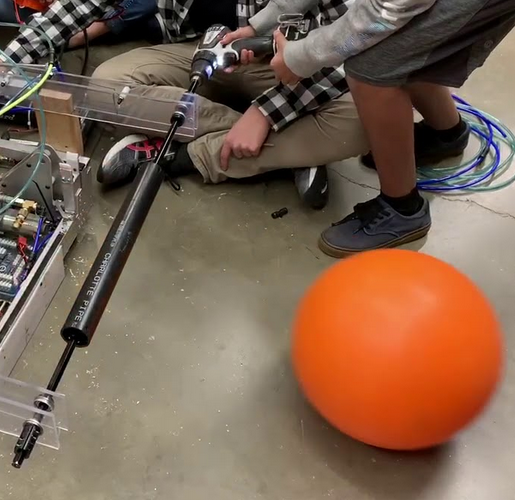
\includegraphics[height=2in]{imgs/intake_beaterbar_1.png}
	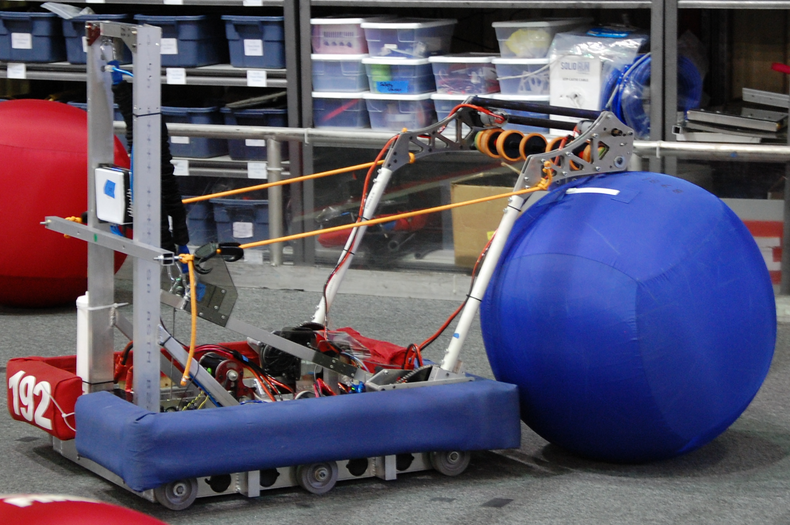
\includegraphics[height=2in]{imgs/intake_beaterbar_2.png}
	\caption{Beater bars.}
\end{figure}

A \textit{beater bar}\index{intake!beater bar} or \textit{horizontal intake axle} has a rotating, grippy element that is horizontal and makes contact with an object, pulling it in. These usually work best with parts that can roll as they enter.

\href{https://www.youtube.com/watch?v=LaoZ8L7H65s}{\color{red}\underline{Video Example}}
\subsection{Side wheels}
\textit{Side wheels} are rotating, grippy elements on a vertical shaft which make contact with an object, pulling it in. These are often spring-loaded to help deal with misalignment as they require somewhat precise positioning (at least more than a beater bar). Because of this, they are typically used where a beater bar is not as viable (like to intake an object that cannot roll).
\subsection{Centering intakes}
\textit{Centering intakes}\index{intake!centering} bring objects in to a particular point.

\begin{figure}[H]
\begin{subfigure}[b]{.45\linewidth}
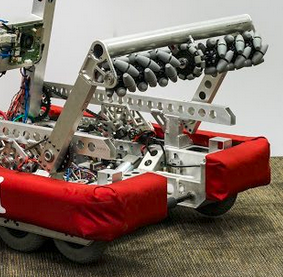
\includegraphics[height=2.1in]{imgs/intake_vectored.png}
\end{subfigure}\begin{subfigure}[b]{.45\linewidth}
\includegraphics[height=2.1in]{imgs/intake_centering.jpeg}
\end{subfigure}
\caption{Left: Vectored intake wheels. Right: Centering intake with belts.}
\end{figure}


\begin{asparaitem}[a)]
\item A simple way of accomplishing this is by creating a beater bar with \textit{Mecanum wheels} or \textit{vectored intake wheels}, which have rollers at a 45 degree angle. They provide a centering action when properly implemented, as the rollers will cause a force vector 45 degrees to the axis of rotation, rather than perpindicular. \href{https://www.youtube.com/watch?v=WwxNSiHXREo}{\color{red}\underline{Video Example}}
\item Multiple belts feeding into each other can also produce the centering effect. \href{https://youtu.be/p0_YOm5fjC8?t=107}{\color{red}\underline{Video Example (1:48)}}
\end{asparaitem}

\subsection{Scoops}
\begin{figure}[H]
	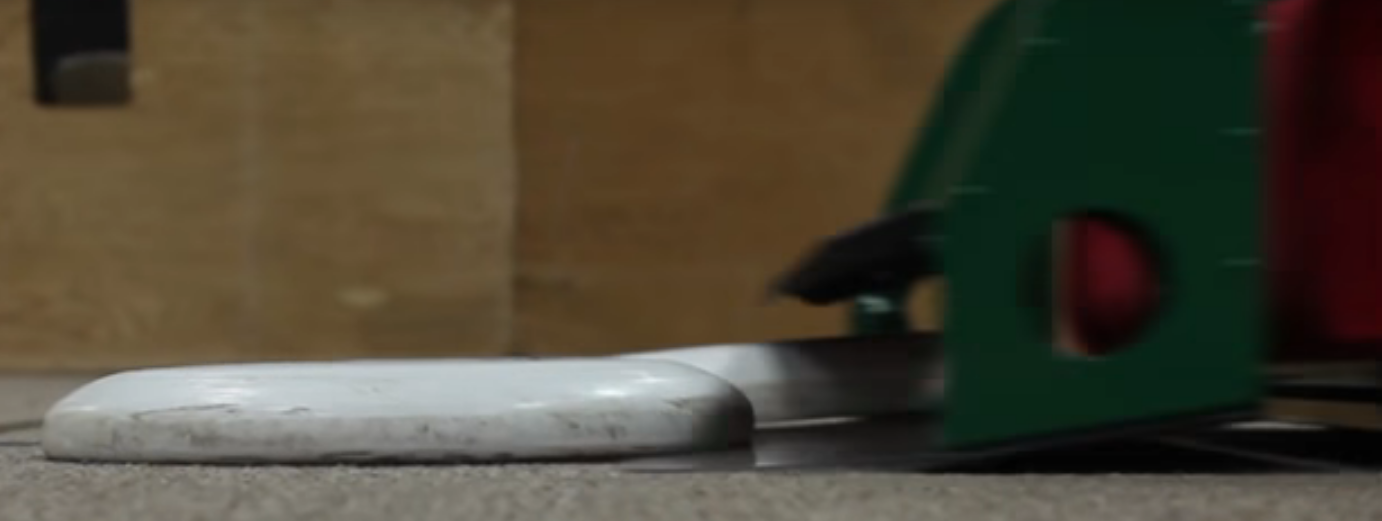
\includegraphics[height=1.5in]{imgs/scoop.png}
	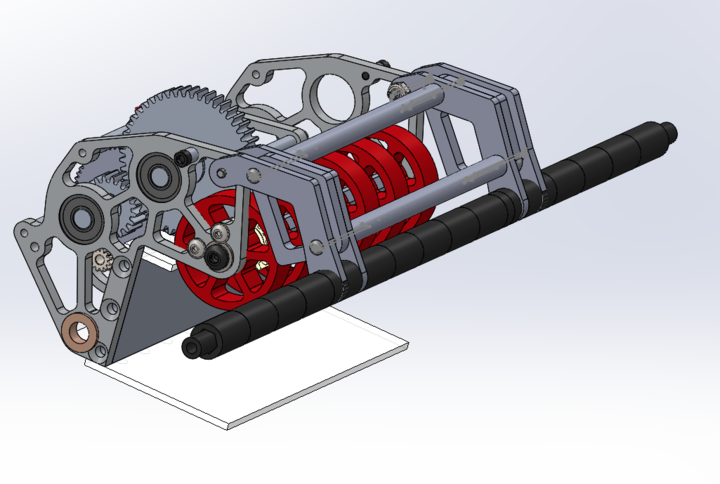
\includegraphics[height=1.5in]{imgs/scoop_roller.png}
	\caption{Left: scoop picking up frisbees. Right: scoop with additional beater bar (in red).}
\end{figure}
A \textit{scoop}\index{intake!scoop} simply wedges under an object, picking it off the ground. Scoops can be useful if the object to be picked up has a tapered bottom that is conducive to this and has much higher friction on the surface it is being picked up from versus the surface of the scoop. \href{https://youtu.be/uKy-IKDq_6o?t=38}{\color{red}\underline{Video Example (0:38)}} Scoops can also be combined with beater bars to provide positive latching of the object to be grabbed.
\subsection{Vacuums}
\begin{figure}[H]
	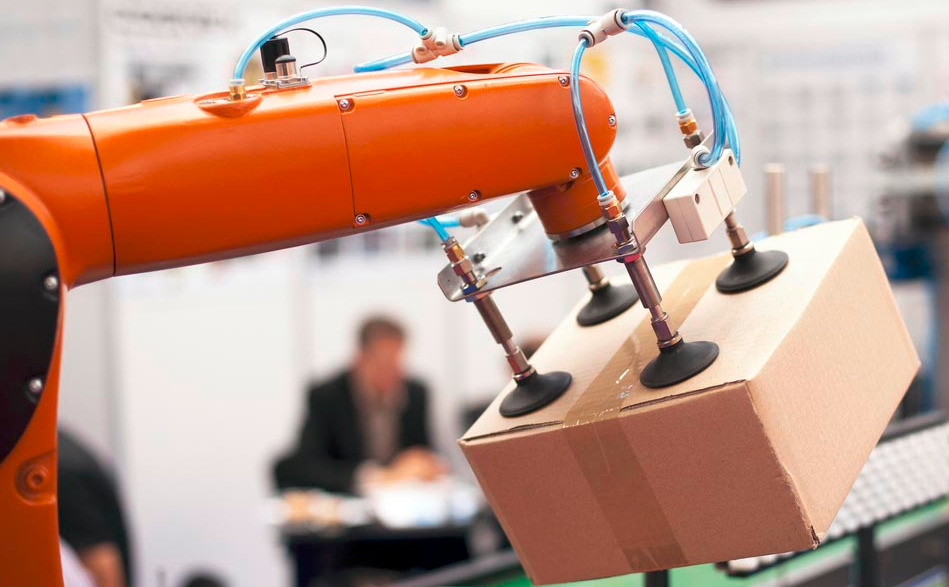
\includegraphics[height=2.3in]{imgs/gripper_vacuum.png}
	\caption{Vacuum gripper on a robot arm lifting a cardboard box.}
\end{figure}
\textit{Vacuum pumps}\index{vacuum} can be used to acquire objects that can form a sufficiently good seal. They are a little difficult to set up properly, and are also notably inefficient and loud, but can be used properly and effectively. \href{https://www.youtube.com/watch?v=T2goz1ghXXk}{\color{red}\underline{Video Example}}

\section{Indexers}
An \textit{indexer}\index{indexer} is any mechanism that takes one or more already-controlled objects and moves them to somewhere else where it can be used.
\subsection{Gravity Hoppers}
\index{hopper}
\begin{figure}[H]
	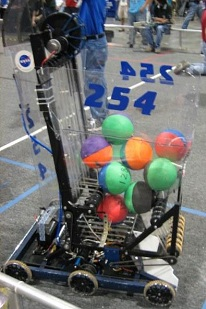
\includegraphics[height=2.3in]{imgs/hopper_gravity_1.jpeg}
	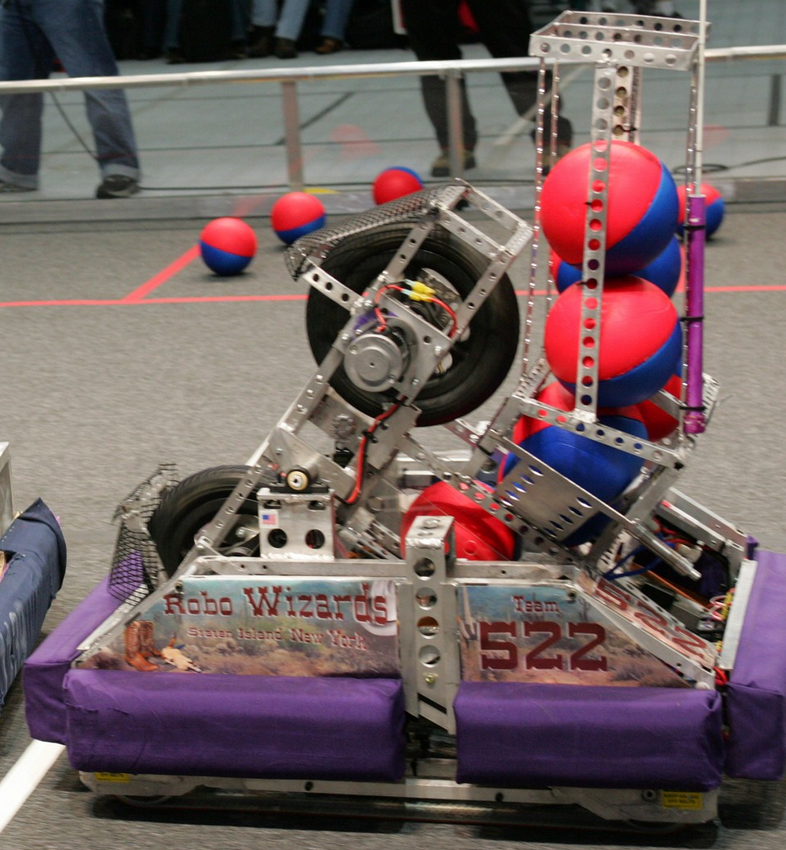
\includegraphics[height=2.3in]{imgs/hopper_gravity_2.png}
	\caption{Gravity hoppers for foam balls.}
\end{figure}
\textit{Gravity-fed, metered hoppers} are the simplest form of indexing. A hopper holds objects, and a wheel or gate controls their exit. Hoppers can jam easily depending on the object, and for high-speed applications, may not feed fast enough on their own.
\subsection{Conveyors}
\begin{figure}[H]
	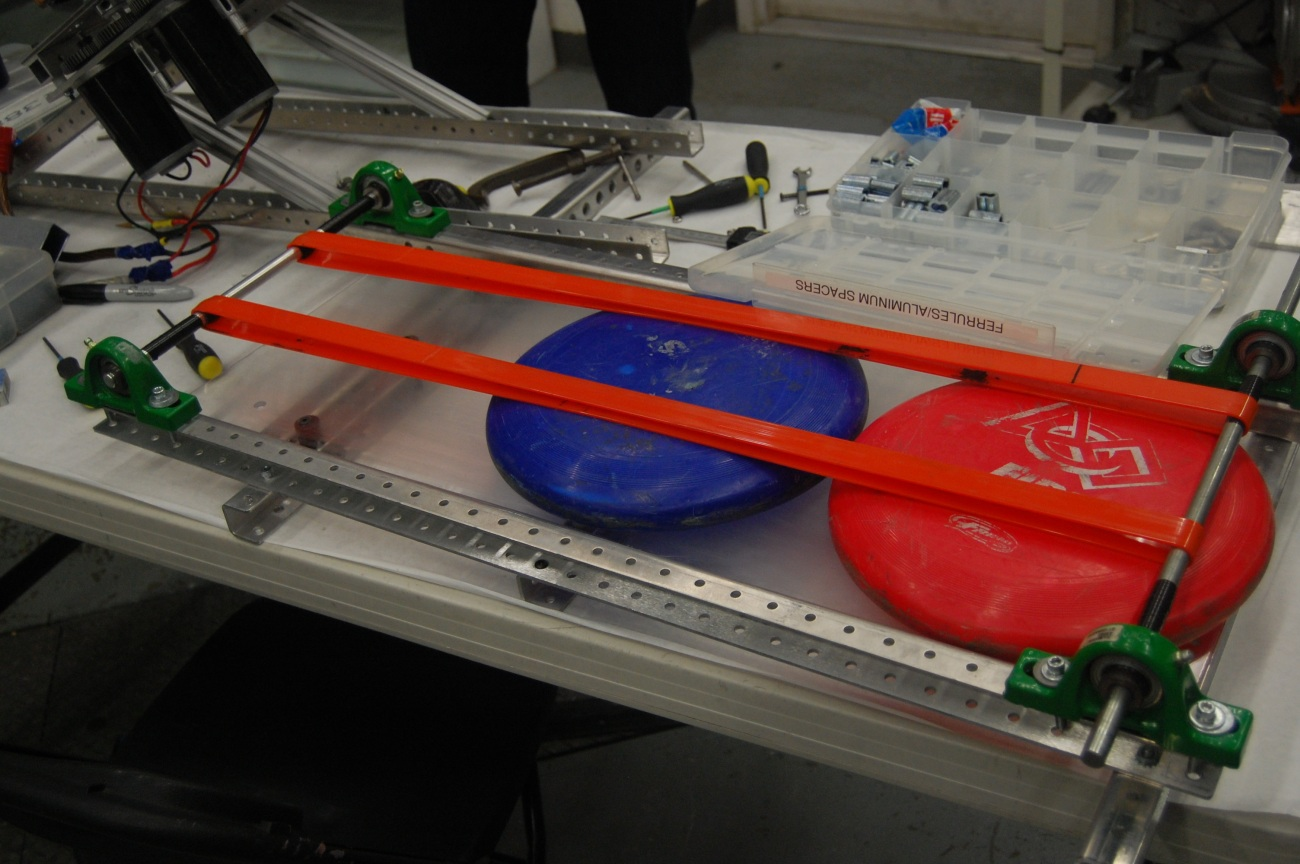
\includegraphics[width=0.8\textwidth]{imgs/conveyor_single.jpeg}
	\caption{A single conveyor belt feeding frisbees from the top.}
\end{figure}
\textit{Conveyors}\index{conveyor} are the most common type of indexer. Objects are fed single file from one place to another using continuous belts. Variants of this exist, such as dual-conveyors (where objects are passed between two conveyors, so they do not need to roll or slide, but are still well-constrained).
\href{https://www.youtube.com/watch?v=by2A56mHdRM}{\color{red}\underline{Video Example}}
\subsection{Rotary Hoppers}
\begin{figure}[H]
	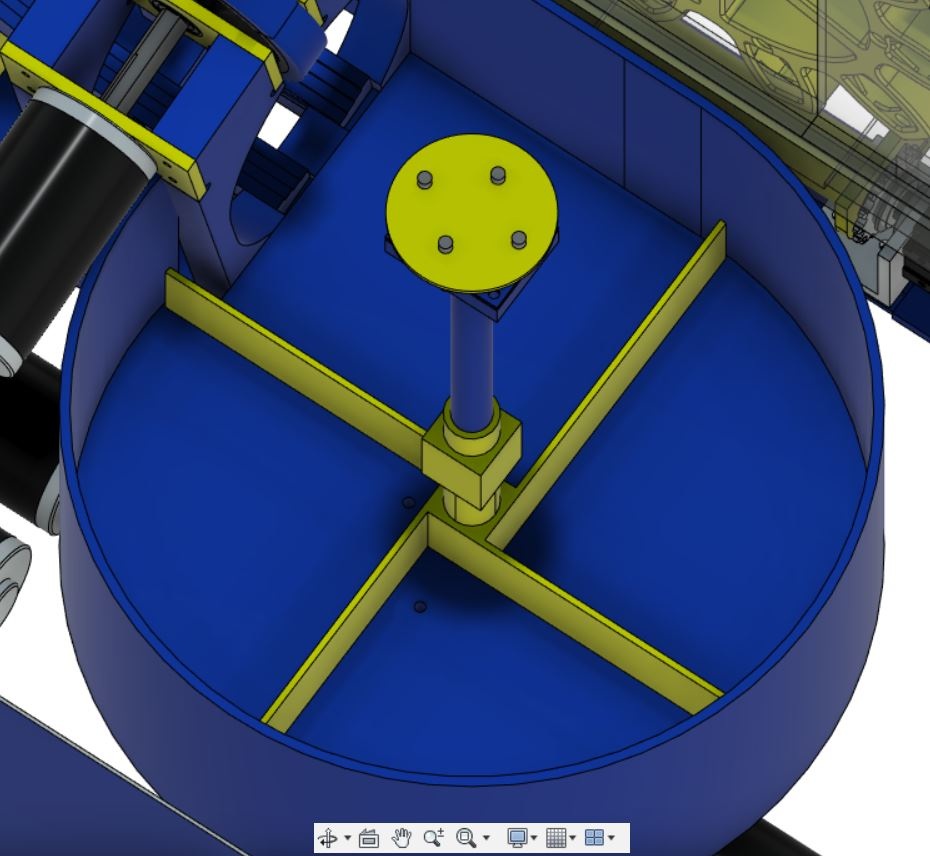
\includegraphics[height=2.3in]{imgs/spindexer.jpeg}
	\caption{Rotary hopper or spindexer}
\end{figure}

\textit{Rotary hoppers}\index{hopper!rotary} or \textit{spindexers}\index{indexer!rotary} are like gravity hoppers, but use some sort of rotating piece at the bottom to both agitate objects in the hopper and forcefully feed them to the next place. These allow for high capacity and control. The base can either have positive interaction with the objects, or frictional interaction (i.e. flat). 


\href{https://youtu.be/ewTCvLp5EUo?t=12}{\color{red}\underline{Video Example (0:12)}}
\subsection{Agitated Hoppers}

\begin{figure}[H]
	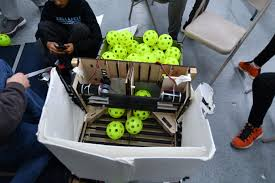
\includegraphics[height=1.8in]{imgs/hopper_agitated_1.jpeg}
	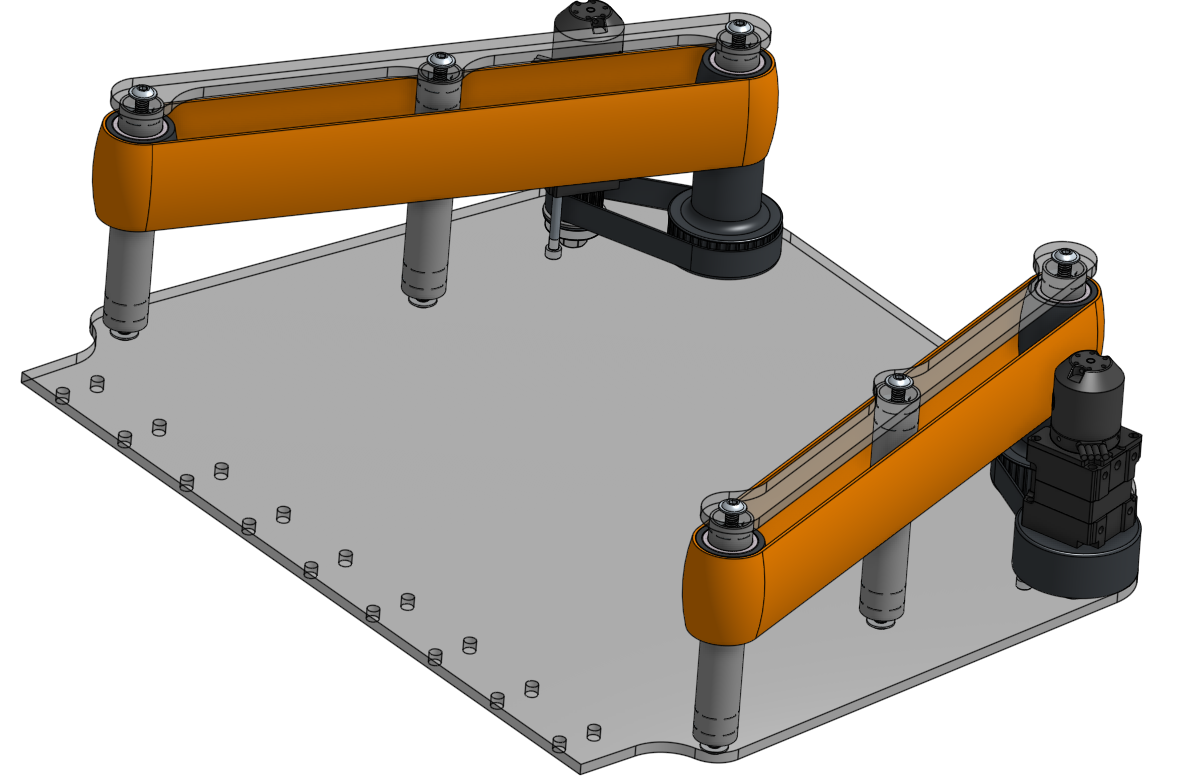
\includegraphics[height=1.8in]{imgs/hopper_agitated_2.png}
	\caption{Agitated hoppers.}
\end{figure}

\textit{Agitated hoppers}\index{hopper!agitated} are slightly angled hoppers which also feature moving sidewalls or rollers that help agitate objects and may even influence them to move faster than gravity would normally allow for. These can be simple to design and integrate while allowing for greater throughput and less jamming than a gravity hopper. 

\href{https://www.youtube.com/watch?v=9vIrTnXu7ho}{\color{red}\underline{Video Example}}
\section{Lifts}

A \textit{lift}\index{lift} is any mechanism that moves things up and down (though they all can be used to move objects in any direction). 

\subsection{Elevators, Cascade and Continuous}
\index{elevator}
\begin{figure}[H]
	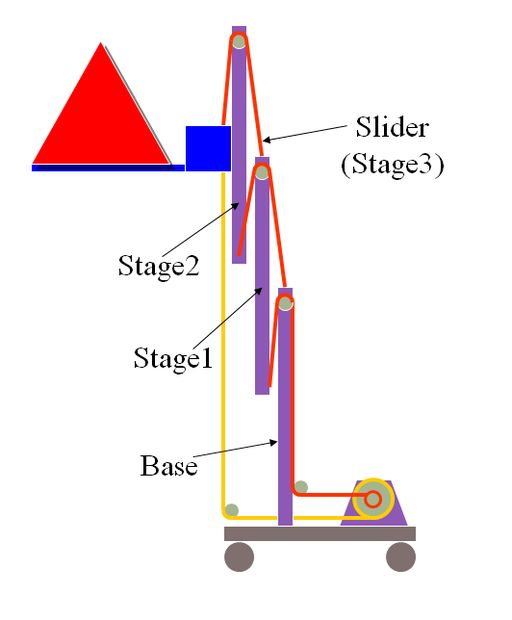
\includegraphics[height=2.1in]{imgs/elevator_cascade.jpeg}
	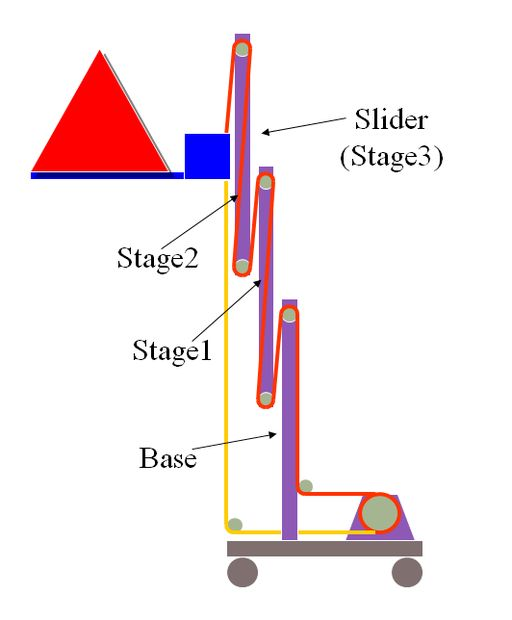
\includegraphics[height=2.1in]{imgs/elevator_continuous.jpeg}
	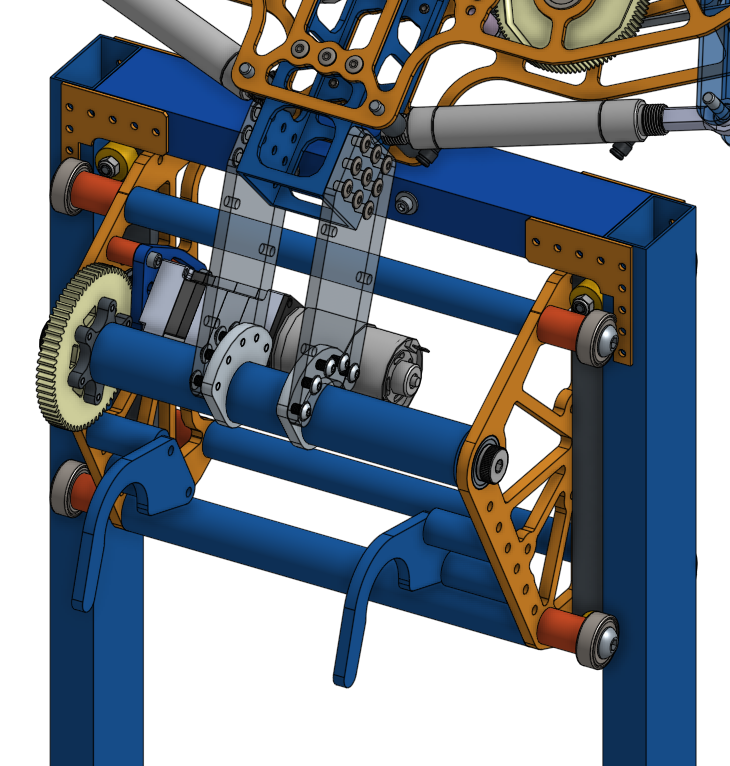
\includegraphics[height=2.1in]{imgs/elevator_construction.png}
	\caption{Elevators- cascade (left) and continuous (middle). Example construction detail on right.}
\end{figure}

An \textit{elevator} is a mechanism that moves back and forth in a straight line. The multiple \textit{stages} are held together with bearings or slides to reduce friction. \textit{Cascade}\index{elevator!cascade vs. continuous} and \textit{Continous} elevators are able to reach further than their initial size without additional degrees of freedom by using special rigging of string to pull multiple stages that are nested in each other.

Cascade elevators have multiple strings to consider. They also have mechanical disadvantage by a factor of the number of stages in the lift. Continuous elevators do not have this mechanical disadvantage and only have one string to worry about.

\href{https://youtu.be/HJVGgaAJefo?t=37}{\color{red}\underline{Video Example (0:37)}}
\subsection{Scissor Lifts}
\begin{figure}[H]
	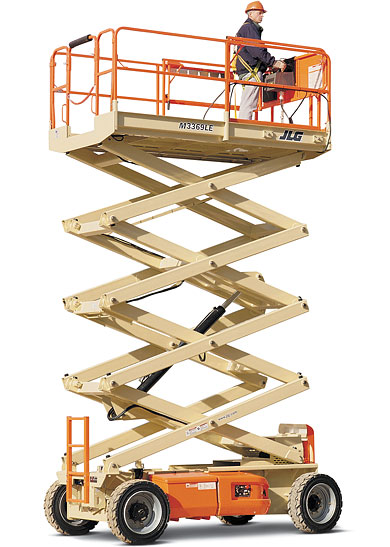
\includegraphics[height=2.5in]{imgs/scissorlift.jpeg}
	\caption{Scissor lifts}
\end{figure}

\textit{Scissor lifts}\index{lift!scissor} are linkages that can achieve incredible extension from a compact initial size. However, they can be quite problematic in practice, as the parts count to create the several stages can be quite high, and because there are so many parts, so is the backlash. They also have incredibly poor mechanical advantage, meaning the force required to drive them is very significant.

\href{https://youtu.be/J_VfCjKBGNw?t=18}{\color{red}\underline{Video Example (0:18)}}
\subsection{Parallel 4 Bar}
\begin{figure}[H]
	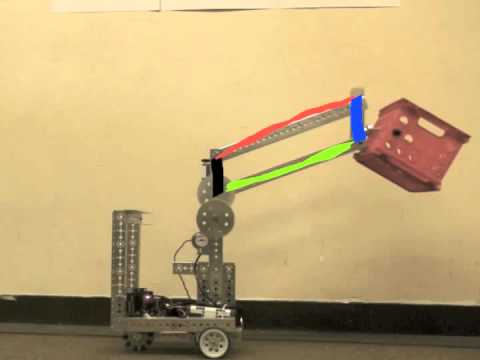
\includegraphics[height=2.5in]{imgs/parallel_4bar.jpeg}
	\caption{Parallel 4 bar mechanism}
\end{figure}

\textit{Parallel 4 bar linkages}\index{4-bar linkage} have four links forming a parallelogram, where two opposing sides are the input and output. These are simple to make but do not lift straight up and down- they will move outwards in an arc as they rise. This may be a desirable trait. \href{https://www.youtube.com/watch?v=hnxqZlG-508}{\color{red}\underline{Video Example 1}} \href{https://youtu.be/LaV0zbKz-Qg?t=36}{\color{red}\underline{Video Example 2 (0:36)}}
\subsection{Virtual 4 Bar}

\begin{figure}[H]
	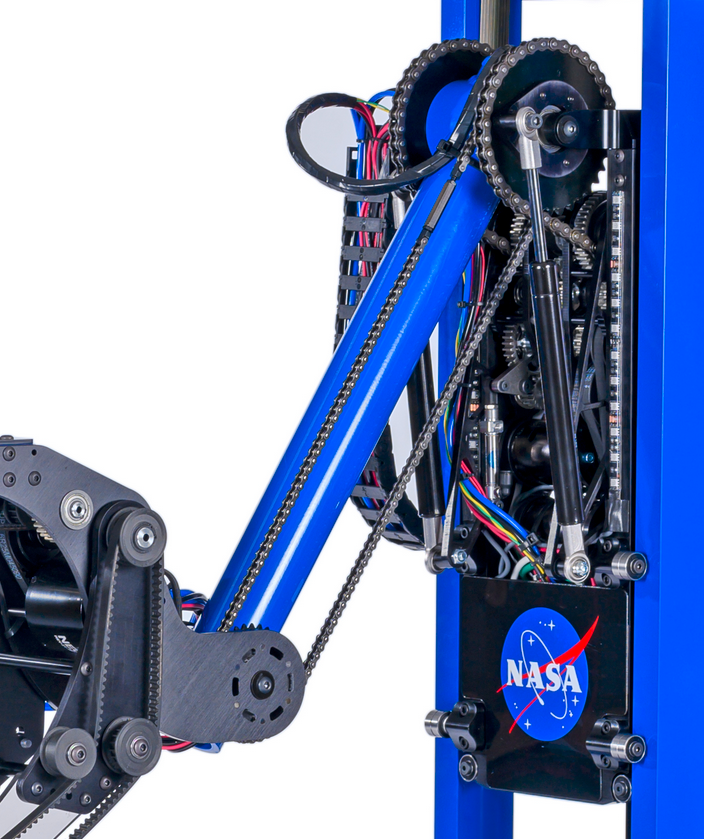
\includegraphics[height=2.5in]{imgs/virtual_4bar_1.png}
	\caption{Virtual 4 bar mechanism}
\end{figure}

\textit{Virtual 4 bars}\index{4-bar linkage!virtual} achieve similar motion to parallel 4 bars, but overcome the major issue regarding the \textit{singularity}\index{singularity} that occurs when the links come to a straight line. At this singularity, the mechanism is no longer fully defined and may invert, causing undesired behavior. Virtual 4 bars, on the other hand, can rotate continuously. They are built by using a single linkage, two sprockets, and chain binding the sprockets together. The sprockets are fixed on either end.

\href{https://www.youtube.com/watch?v=nH6P4BcwtiE}{\color{red}\underline{Video Example}}

\subsection{2N Bar}

\begin{figure}[H]
	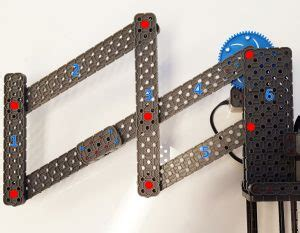
\includegraphics[height=2.5in]{imgs/6bar.jpeg}
	\caption{6 bar linkage.}
\end{figure}

4 bars take up a lot of dead space. They can be made to extend further by staging multiple of them together. These may be called \textit{6 bars}\index{6 bar linkage}, \textit{8 bars}\index{8 bar linkage}, and so forth- there is no theoretical upper limit, but increasing the number of stages will pose the same issues as a scissor lift will (you may note, that the underlying linkages are nearly identical, they are just used differently).

\href{https://www.youtube.com/watch?v=twwNv4easgk}{\color{red}\underline{Video Example}}

\subsection{Double Reverse 4 Bar}

\begin{figure}[H]
	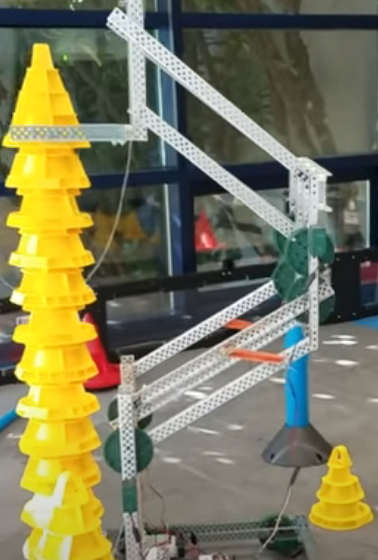
\includegraphics[height=2.5in]{imgs/double_reverse_4bar.png}
	\caption{Double-reverse 4 bar.}
\end{figure}

\textit{Double reverse 4 bars}\index{4-bar linkage!double-reverse} sound complicated, and they are to some degree. These are two 4 bar mechanisms stacked on top of each other, reversed, and linked together (either with gears or a link). This allows them to fold up flat but reach tall heights, and move in a straight line (as any inward motion by the lower 4-bar is counteracted by the outward motion of the upper 4-bar).

\href{https://www.youtube.com/watch?v=iFq8dKUZOww}{\color{red}\underline{Video Example}}

%\section{Latches}
%\textit{Latches}\index{Latches} grab onto things and don't let go.
%\subsection{Latches}
%\subsection{Overcenter mechanisms}

\subsection{Counterbalancing}
\index{counterbalance} 
\begin{figure}[H]
	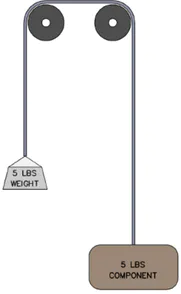
\includegraphics[height=2in]{imgs/counterbalance.png}
	\caption{A counterbalance.}
\end{figure}

Any lift may be improved by the use of a \textit{counterbalance}. The purpose of a counterbalance is to provide load that counteracts the normally seen load or weight. This way force exerted on the lift is used not to fight gravity, but to accelerate the mass of the system. Because weight is usually a concern (and adding mass would increase the inertial loads of the system), a \textit{counterspring} may be used to offset the load without much added mass. Constant-force springs are particularly equipped for this task as they can extend a great distance and provide constant force rather than counterweight that varies with position.

\section{Shooters}
\textit{Shooters}\index{shooter} take objects and propel them great distances.
\subsection{Flywheel-Based Shooter}
\textit{Flywheel based launchers} store energy in \textit{flywheels}\index{flywheel} spinning at high velocity. Objects can then be introduced to the flywheels, and the energy is transferred via friction to the objects. This makes flywheel based launchers good for high-throughput applications.

\begin{figure}[H]
	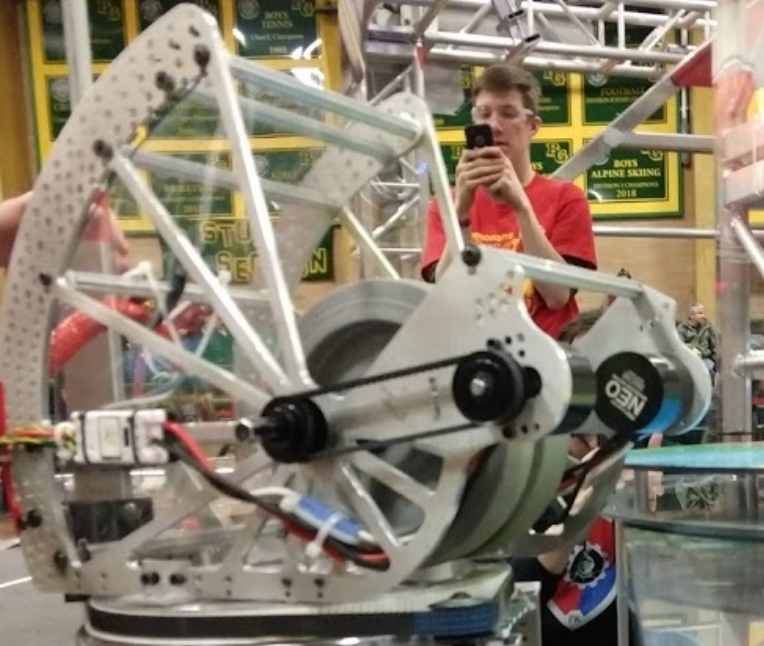
\includegraphics[height=2.2in]{imgs/shooter_hooded.png}
	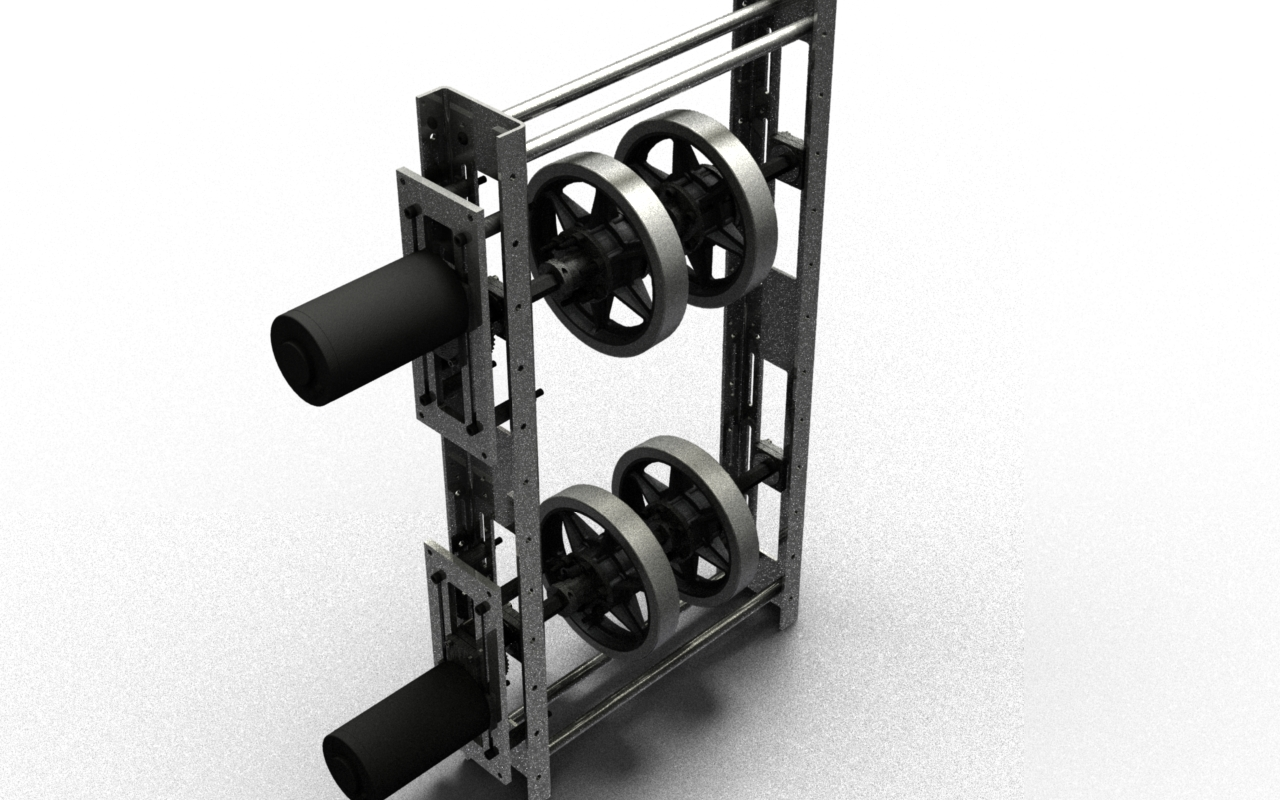
\includegraphics[height=2.2in]{imgs/shooter_dualwheel.jpeg}
	\caption{Wheeled shooters. Left: hooded. Right: dual-wheel.}
\end{figure}

\textit{Hooded} shooters use a singular set of wheels and a fixed \textit{hood} to contact the ball. This produces a high amount of backspin, which may be desirable due to the \textit{Magnus effect} which generates lift (or drop) on spinning objects.

\textit{Opposed wheel} shooters use mutiple sets of wheels to contact the ball. This allows for control over backspin, and may be easier to package. \href{https://youtu.be/pgMU_AxzxAE?t=67}{\color{red}\underline{Example Video (In Slow-Mo!) (1:07)}}

Flywheel based shooters sometimes have multiple stages of flywheels in order to accelerate the ball over a longer period of time. Belts can also be used to achieve the same principle.
\subsection{Catapults and Punches}
\textit{Catapults}\index{shooter!catapult} and \textit{punches}\index{shooter!punch} store energy in by pulling back springs or compressing air. Catapults work as a lever arm while punches work linearly, but both use this stored energy to accelerate a sled or cradle containing the object to be launched.

\begin{figure}[H]
\begin{subfigure}[b]{.32\linewidth}
	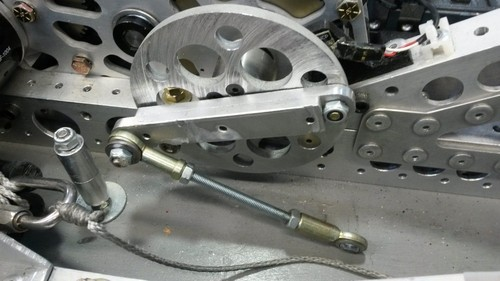
\includegraphics[height=1.8in]{imgs/choo_choo.jpeg}
	\caption{Choo-choo}
\end{subfigure}\begin{subfigure}[b]{.32\linewidth}
	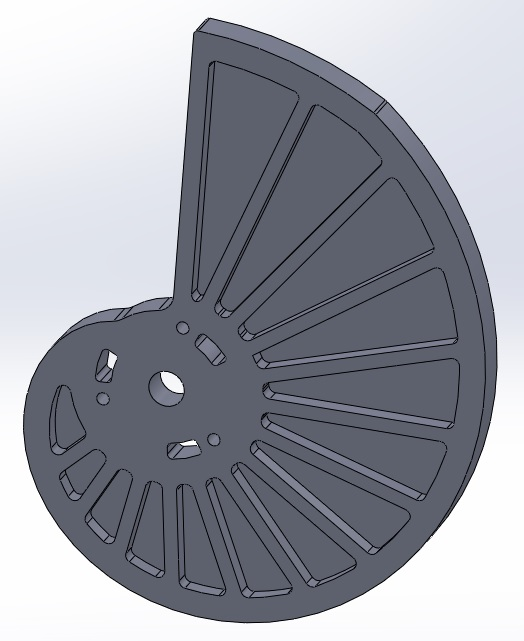
\includegraphics[height=1.8in]{imgs/snail_cam.jpeg}
	\caption{Snail cam}
\end{subfigure}
\end{figure}

\begin{asparaenum}[a)]
\item A \textit{choo-choo}\index{choo-choo} uses a rotating plate with a pin, a link, and another link or string. As the plate is rotated, the pin makes contact with the link. Eventually the second link/string gets pulled back and goes over-center from this pin, so that the pin no longer supports the link. At this point the spring pulls the mechanism forwards as it fires. \href{https://www.youtube.com/watch?v=Kh-PVMSF7VU}{\color{red}\underline{Video Example}}
%SIDEBAR: THIS IS REALLY COOL https://www.youtube.com/watch?v=aIDwkuRAjqs

\item \textit{Snail cams}\index{snail cam} can be used to pull back the sled/cradle, and as the cam continues moving, it eventually returns to its starting point, causing the sled/cradle to fly forth.

\item In a \textit{winch and release}\index{winch and release} a winch pulls back the sled/cradle. When firing is desired, a release mechanism (like those discussed in section \ref{section:disengagement}) allows the sled/cradle to fly forth. \href{https://www.youtube.com/watch?v=YFmG_b4B-BE}{\color{red}\underline{Video Example}}

\item \textit{Pneumatic cylinders}\index{pneumatic cylinder} are very simple ways of creating sudden bursts of energy. \href{https://youtu.be/1QOYdA5IPJQ?t=81}{\color{red}\underline{Video Example (1:21)}}
\end{asparaenum}

%TODO: Do these
%\subsection{Flicker launchers}
%\subsection{Throwers}

\section{Drivetrains} \label{section:drivetrains}
Drivetrains allow for movement across surfaces. Drivetrains have many considerations which depend on the use case.
\begin{asparaenum}[a)]
\item The type of \textit{microterrain}\index{terrain} that must be traversed has to be considered- is it squishy? Is it solid? Is it slippery or icy? 
\item The type of \textit{macroterrain} that must be traversed has to be considered- is it flat? Is it bumpy? What is the geometry of the bumps that must be traversed- will the drivetrain \textit{bottom out} or \textit{high-center}?
\item There may be a \textit{target velocity} that must be reached.
\item The \textit{ride quality} is important so as not to damage cargo, electronics, or passengers.
\item The \textit{cycle time}\index{cycle} or \textit{lap time} is a factor for sport applications.
\item The \textit{efficiency}\index{efficiency} or \textit{energy consumption} may be a factor.
\item The required \textit{degrees of freedom}\index{degrees of freedom} are often important- is straight line movement OK? Is steered drive enough? Do you need to turn on a dime? Do you need to move \textit{omnidirectionally}\index{omnidirectional} (in any direction without a change in pose)?
\item \textit{Traction}\index{traction}, whether to climb a steep hill, push objects, or remain in place, is a very important consideration.
\end{asparaenum}
\subsection{Car Steering}
\begin{figure}[H]
	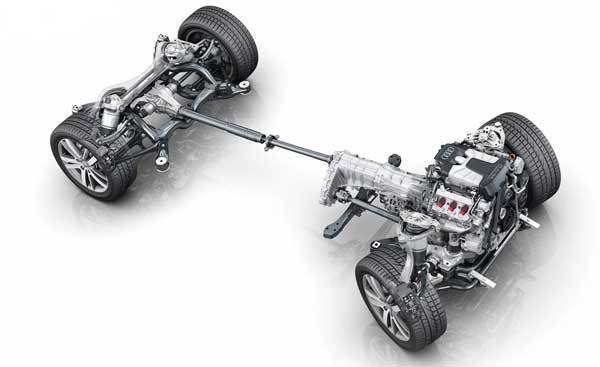
\includegraphics[width=0.8\textwidth]{imgs/drivetrain_car.jpeg}
	\caption{Drivetrain of a car}
\end{figure}

The key aspects of a conventional car's drivetrain are:
\begin{asparaenum}
	\item Either the front or rear axle is powered. The left and right tires are powered by the same degree of freedom.
	\item The front wheels are steered, usually up to 60 degrees.
\end{asparaenum}

This means that the car has 1.5 degrees of freedom. The car can move forwards and backwards (one degree of freedom), and while it is moving forwards and backwards, it can change its direction by steering (a half degree of freedom). This may sound limited, but the simplicity of the setup makes it conducive to designing in other complexities that are more important in many scenarios, such as a suspension to achieve superior ride quality.

\subsection{Differential Drives}
\begin{figure}[H]
	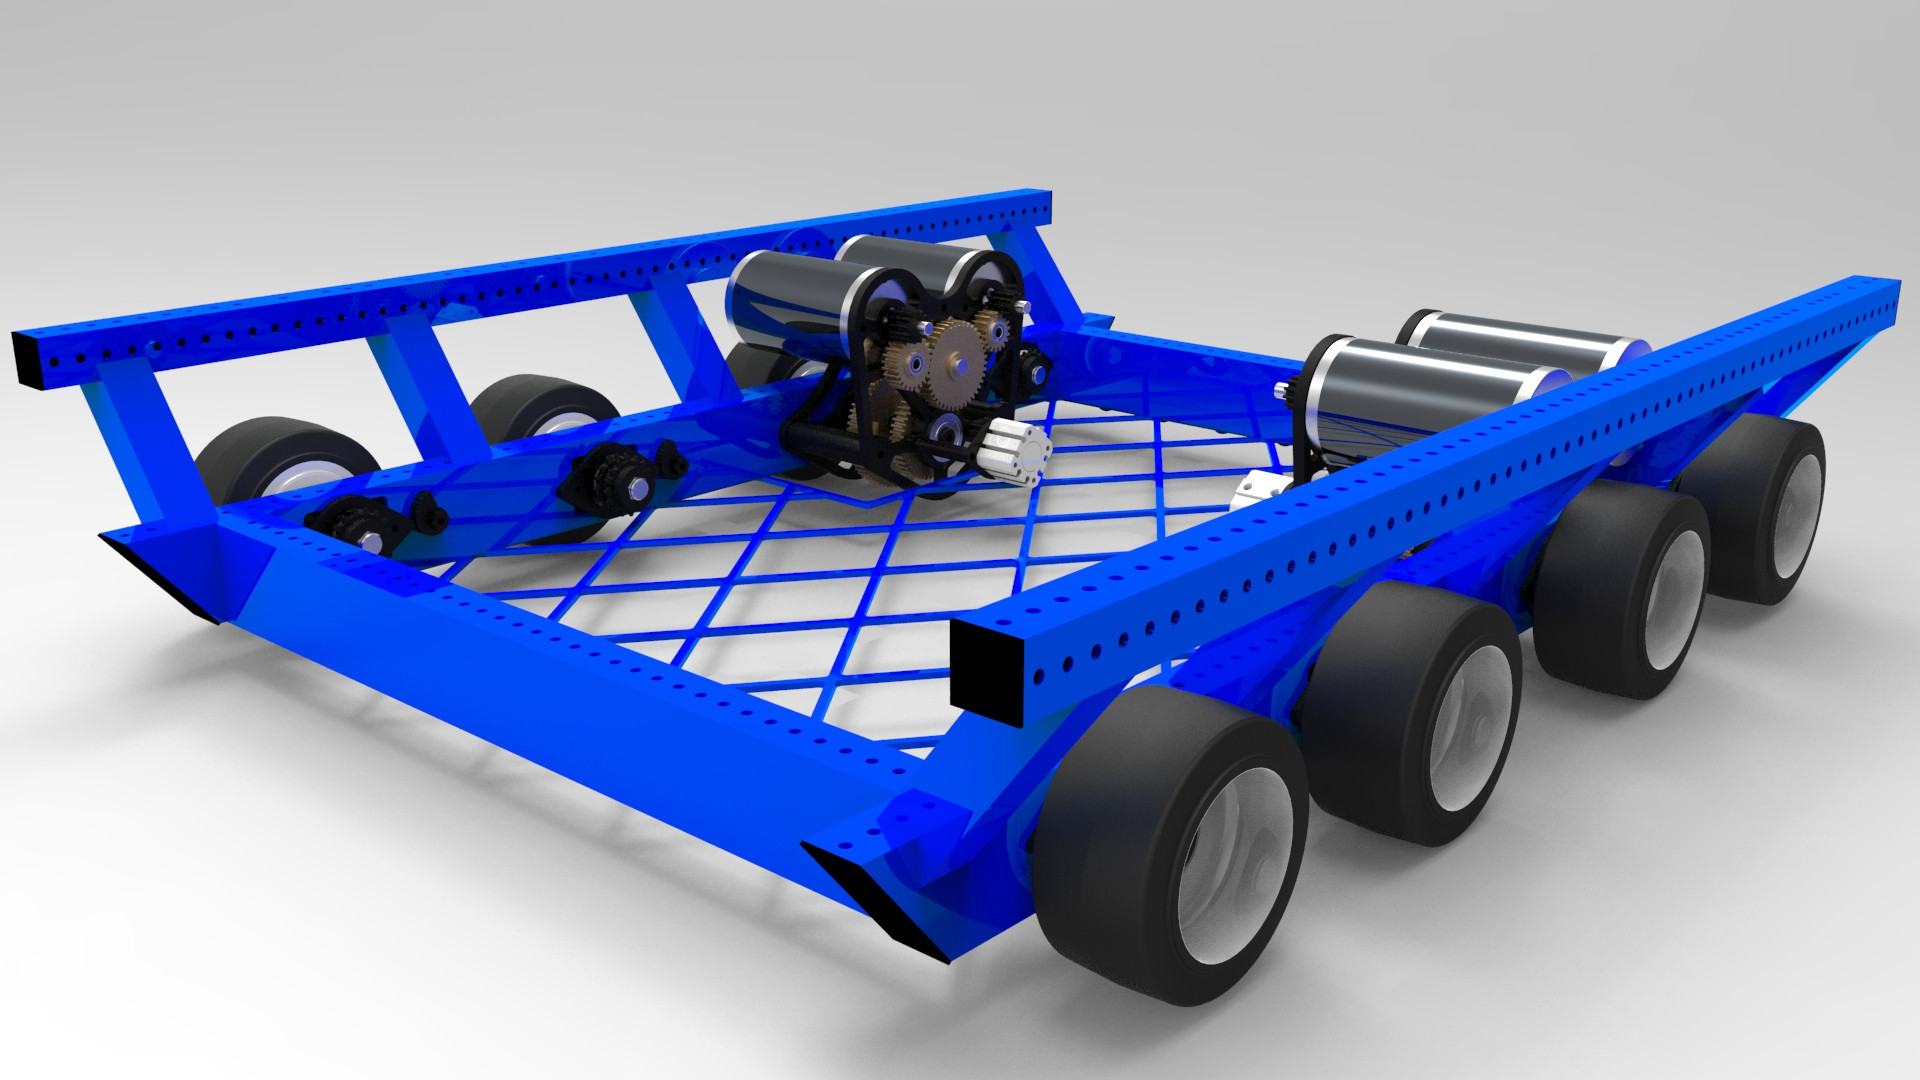
\includegraphics[width=0.8\textwidth]{imgs/drivetrain_differential.jpeg}
	\caption{Differential drive.}
\end{figure}

\textit{Differential drives}\index{differential drive} (which do not necessarially have \textit{differential gearsets}), often called \textit{tank drives} (even if they don't have tank-style treads) have two sets of wheels (or treads) that are controlled to move independent of each other.

\begin{figure}[H]
\begin{subfigure}[b]{.3\linewidth}
	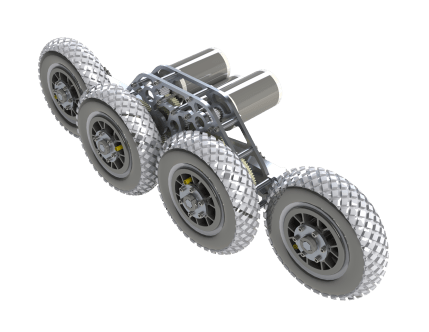
\includegraphics[height=1.45in]{imgs/drivetrain_pneumatic.png}
\end{subfigure}\begin{subfigure}[b]{.6\linewidth}
	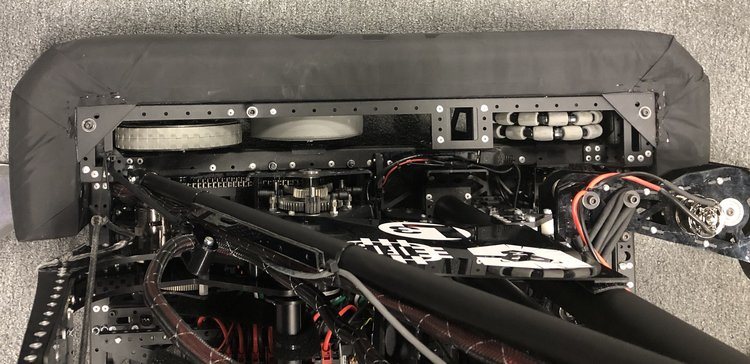
\includegraphics[height=1.45in]{imgs/drivetrain_148_2018.jpeg}
\end{subfigure}

\begin{subfigure}[b]{.45\linewidth}
	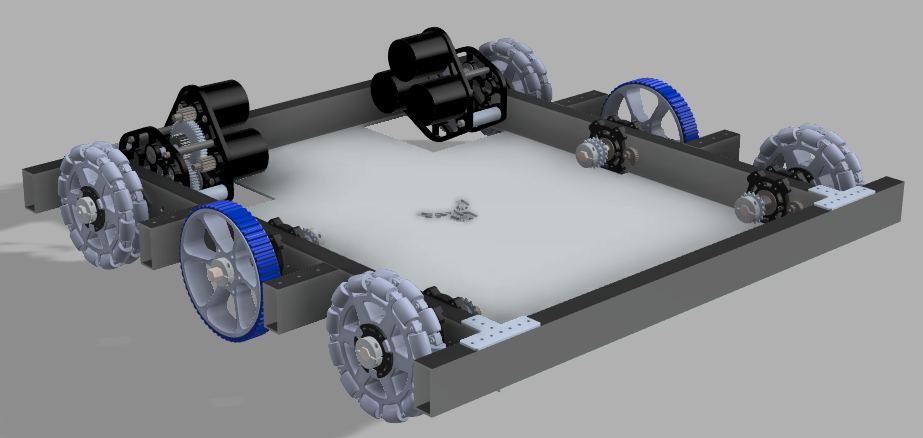
\includegraphics[height=1.4in]{imgs/drivetrain_corneromni.png}
\end{subfigure}\begin{subfigure}[b]{.45\linewidth}
	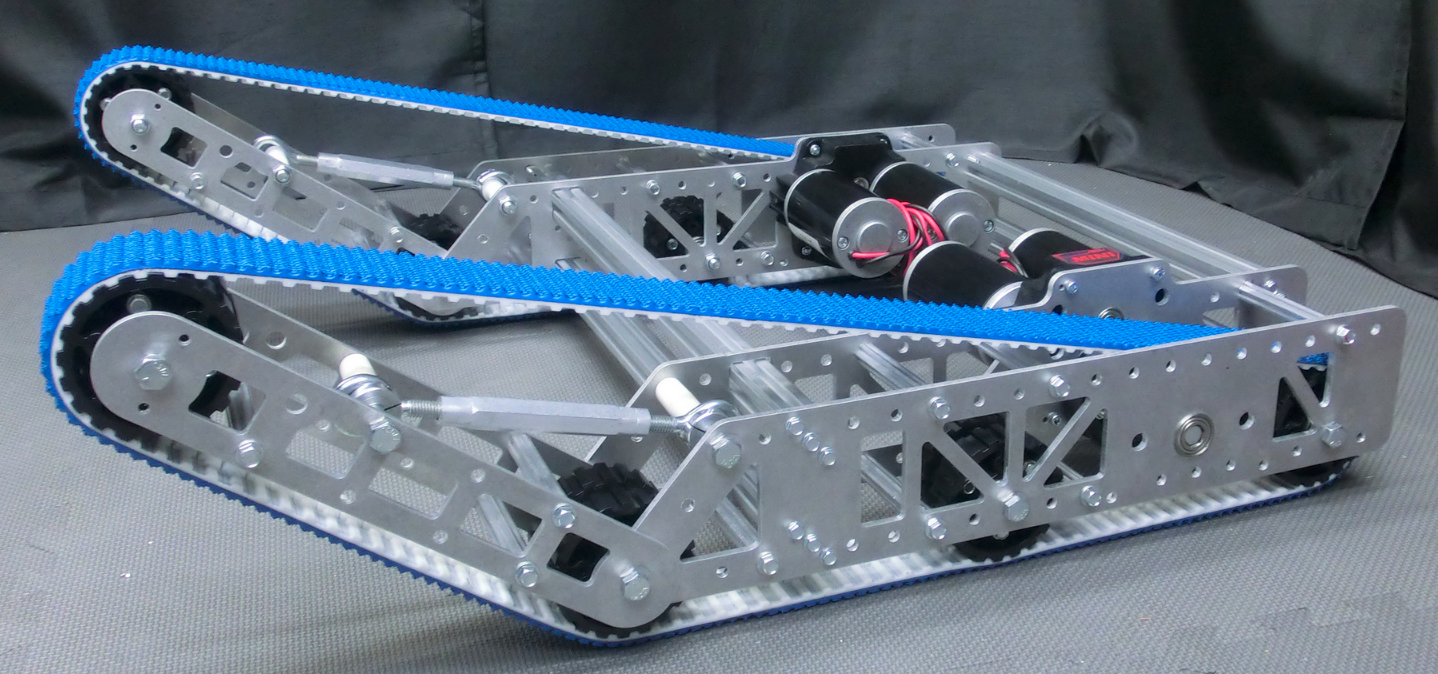
\includegraphics[height=1.4in]{imgs/drivetrain_tank.png}
\end{subfigure}
\caption{Various differential drives.}
\end{figure}

Sizes, types, amounts, and positioning may be mixed and matched to achieve different goals like climbing obstacles or additional maneuverability.

One parameter that isn't obviously shown is the \textit{center drop} \index{differential drive!drop center}. All differential drives have \textit{turning scrub} \index{wheel!scrub} or \textit{wheel slip} that happens when the wheels scrub against the ground sideways.



\begin{figure}[H]
\begin{subfigure}[]{0.5\linewidth}
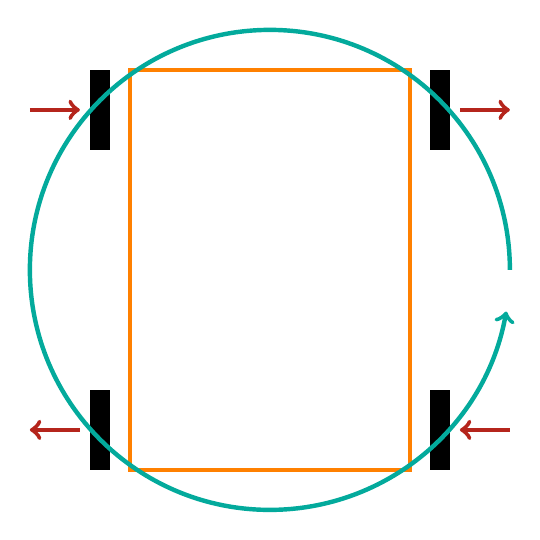
\begin{tikzpicture}[x=1in, y=1in]
	\draw[orange, ultra thick] (-0.7,-1)--(-0.7,1)--(0.7,1)--(0.7,-1)--cycle;
	\fill[black] (-0.9,0.6)--(-0.8,0.6)--(-0.8,1.0)--(-0.9,1.0)--cycle;
	\fill[black] (0.9,0.6)--(0.8,0.6)--(0.8,1.0)--(0.9,1.0)--cycle;
	\fill[black] (-0.9,-0.6)--(-0.8,-0.6)--(-0.8,-1.0)--(-0.9,-1.0)--cycle;
	\fill[black] (0.9,-0.6)--(0.8,-0.6)--(0.8,-1.0)--(0.9,-1.0)--cycle;
	\draw[JungleGreen, ultra thick, ->] (1.2,0) arc (0:350:1.2);
	
	\draw[BrickRed, ultra thick, ->] (-1.2,0.8)--(-0.95,0.8);
	\draw[BrickRed, ultra thick, ->] (0.95,0.8)--(1.2,0.8);
	\draw[BrickRed, ultra thick, ->] (-0.95,-0.8)--(-1.2,-0.8);
	\draw[BrickRed, ultra thick, ->] (1.2,-0.8)--(0.95,-0.8);
\end{tikzpicture}
\end{subfigure}\begin{subfigure}[]{0.5\linewidth}
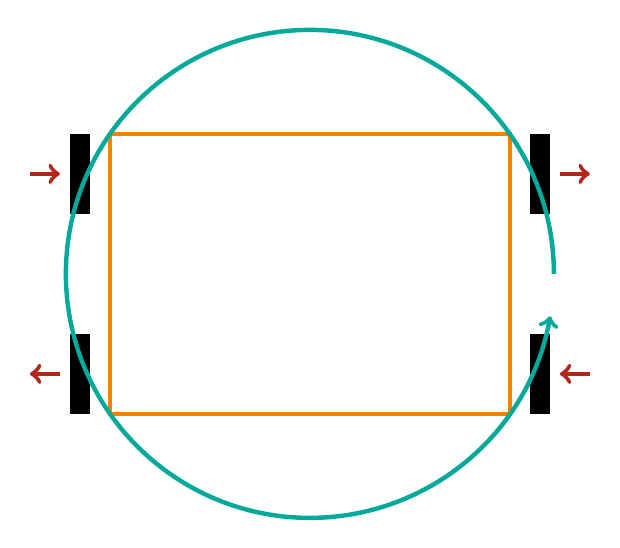
\begin{tikzpicture}[x=1in, y=1in]
	\draw[orange, ultra thick] (-1,-0.7)--(-1,0.7)--(1,0.7)--(1.0,-0.7)--cycle;
	\fill[black] (-1.2,0.3)--(-1.1,0.3)--(-1.1,0.7)--(-1.2,0.7)--cycle;
	\fill[black] (1.2,0.3)--(1.1,0.3)--(1.1,0.7)--(1.2,0.7)--cycle;
	\fill[black] (-1.2,-0.3)--(-1.1,-0.3)--(-1.1,-0.7)--(-1.2,-0.7)--cycle;
	\fill[black] (1.2,-0.3)--(1.1,-0.3)--(1.1,-0.7)--(1.2,-0.7)--cycle;
	\draw[JungleGreen, ultra thick, ->] (1.22,0) arc (0:350:1.22);
	
	\draw[BrickRed, ultra thick, ->] (-1.4,0.5)--(-1.25,0.5);
	\draw[BrickRed, ultra thick, ->] (1.25,0.5)--(1.4,0.5);
	\draw[BrickRed, ultra thick, ->] (-1.25,-0.5)--(-1.4,-0.5);
	\draw[BrickRed, ultra thick, ->] (1.4,-0.5)--(1.25,-0.5);
\end{tikzpicture}
\end{subfigure}

\caption{Top view of turning scrub (red arrows) of two drivetrains while turning.}
\end{figure}

When the aspect ratio of the differential drive is wider than longer, the turning scrub is reduced, making turning much easier. However, this causes the drivetrain to be more prone to tipping in the fore-aft direction. If we drop the center wheel(s) of a drivetrain, we can cause the drivetrain to have the full potential set of wheels it would need to be stable while giving it an aspect ratio conducive to turning.

\begin{figure}[H]
\begin{subfigure}[]{0.45\linewidth}
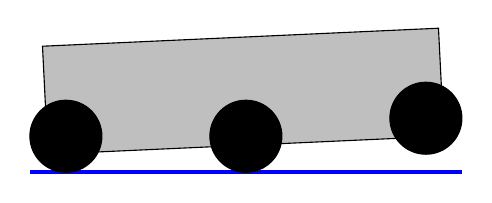
\begin{tikzpicture}[x=0.9in, y=0.9in]
	\draw[blue, ultra thick] (-1.2,-.25)--(+1.2,-.25);
	\filldraw[black, fill=lightgray] (-1.1,-0.15)--(1.1,-0.05)--(1.07,0.55)--(-1.13,0.45)--cycle;
	\filldraw[black, fill=black] (-1,-0.05) circle (0.2);
	\filldraw[black, fill=black] (0,-0.05) circle (0.2);
	\filldraw[black, fill=black] (+1,0.05) circle(0.2);
\end{tikzpicture}
\end{subfigure}\begin{subfigure}[]{0.45\linewidth}
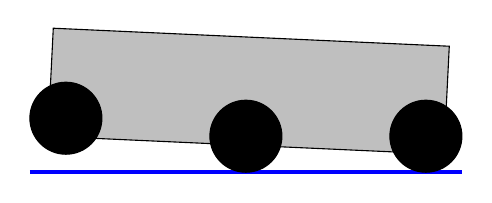
\begin{tikzpicture}[x=0.9in, y=0.9in]
	\draw[blue, ultra thick] (-1.2,-.25)--(+1.2,-.25);
	\filldraw[black, fill=lightgray] (-1.1,-0.05)--(1.1,-0.15)--(1.13,0.45)--(-1.07,0.55)--cycle;
	\filldraw[black, fill=black] (-1,0.05) circle (0.2);
	\filldraw[black, fill=black] (0,-0.05) circle (0.2);
	\filldraw[black, fill=black] (+1,-0.05) circle(0.2);
\end{tikzpicture}
\end{subfigure}
\caption{Side view of dropped-center drivetrain rocking fore-aft. Center drop is exaggerated.}
\end{figure}

Center drops are usually somewhere between 1/16"-1/8" per 10 inches of drivetrain length, depending on the exact surfaces and wheels being used.

But there's one thing we're leaving out of the picture, and that's the \textit{center of gravity} (CG) \index{center of gravity}. This is the point of the machine where mass is evenly distributed about, and is the 'natural' rotation point. Rotating about this point requires the least amount of effort- rotating  about any other point would cause additional acceleration.

\begin{figure}[H]
\begin{subfigure}[]{0.5\linewidth}
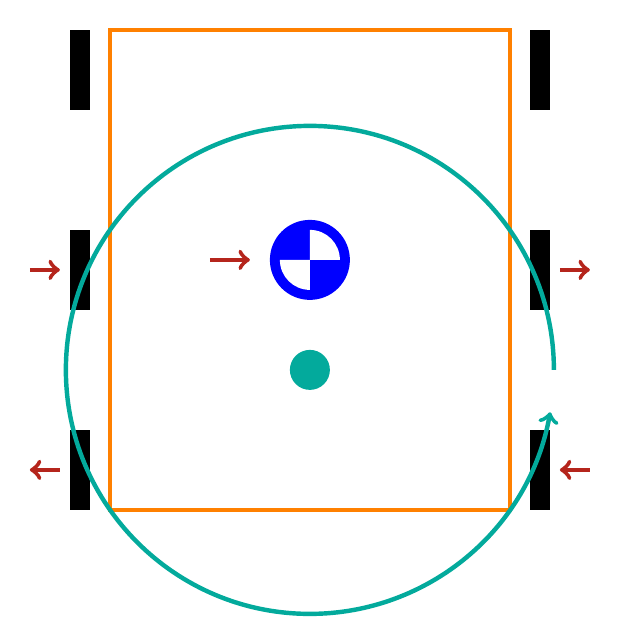
\begin{tikzpicture}[x=1in, y=1in]
	\draw[orange, ultra thick] (-1,-0.7)--(-1,1.7)--(1,1.7)--(1.0,-0.7)--cycle;
	\fill[black] (-1.2,0.3)--(-1.1,0.3)--(-1.1,0.7)--(-1.2,0.7)--cycle;
	\fill[black] (1.2,0.3)--(1.1,0.3)--(1.1,0.7)--(1.2,0.7)--cycle;
	\fill[black] (-1.2,1.3)--(-1.1,1.3)--(-1.1,1.7)--(-1.2,1.7)--cycle;
	\fill[black] (1.2,1.3)--(1.1,1.3)--(1.1,1.7)--(1.2,1.7)--cycle;
	\fill[black] (-1.2,-0.3)--(-1.1,-0.3)--(-1.1,-0.7)--(-1.2,-0.7)--cycle;
	\fill[black] (1.2,-0.3)--(1.1,-0.3)--(1.1,-0.7)--(1.2,-0.7)--cycle;
	\draw[JungleGreen, ultra thick, ->] (1.22,0) arc (0:350:1.22);
	
	\draw[BrickRed, ultra thick, ->] (-1.4,0.5)--(-1.25,0.5);
	\draw[BrickRed, ultra thick, ->] (1.25,0.5)--(1.4,0.5);
	\draw[BrickRed, ultra thick, ->] (-1.25,-0.5)--(-1.4,-0.5);
	\draw[BrickRed, ultra thick, ->] (1.4,-0.5)--(1.25,-0.5);
	
	\fill[JungleGreen] (0,0) circle (0.1);
	\fill[Blue] (0,0.55) circle (0.2);
	\fill[white] (0,0.55)--(0.15,0.55) arc (0:90:0.15)--cycle;
	\fill[white] (0,0.55)--(-0.15,0.55) arc (180:270:0.15)--cycle;
	\draw[BrickRed, ultra thick, ->] (-0.5,0.55)--(-0.3,0.55);
\end{tikzpicture}
\end{subfigure}
\caption{Turning of a drivetrain with center drop. The CG is marked in blue with a standard symbol for CG. The center of rotation is noted with a green dot.}
\end{figure}

Our drop-center drivetrain will alternate between these two suboptimal centers of rotation. Some people don't like this, and thusly opt for an \textit{eight-wheel drive} (8WD). This way the center 4 wheels are normally in contact with the floor, so the center of gravity is very close to the center of rotation.

An alternative (or additional remedy) to adding center drop is to add \textit{corner omnis} \index{wheels!omni}. Instead of the outside wheels being traction wheels, they are omni wheels. These have no resistance to turning scrub, so eliminate scrub entirely. Some designers opt to replace all of the wheels with omnis to make \textit{4 omni drivetrains}. These can produce very agile drifting maneuvers, but have no resistance to being pushed sideways.

\subsection{Omnidrives}
\index{omnidirectional}
\textit{Omnidrives}\index{omnidrive} use wheels with rollers like those described in section \ref{section:wheels} to achieve simultaneous forwards-backwards, left-right, and rotational motion. The wheels limit their use to relatively clean, firm floors, and also limit the materials that can be used on the rollers and thusly their maximum traction.

\begin{figure}[H]
\begin{subfigure}[b]{.45\linewidth}
	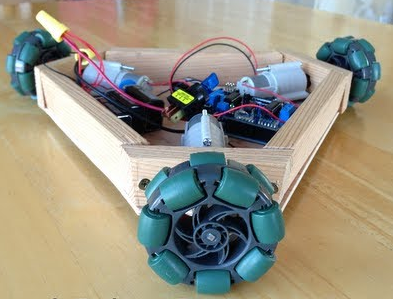
\includegraphics[height=1.7in]{imgs/drivetrain_kiwi.png}
	\caption{Kiwi}
\end{subfigure}\begin{subfigure}[b]{.45\linewidth}
	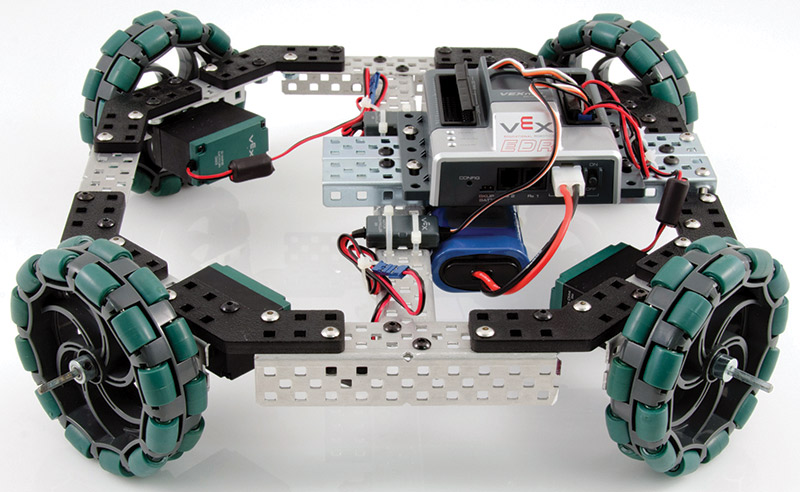
\includegraphics[height=1.7in]{imgs/drivetrain_killough.jpeg}
	\caption{X-drive}
\end{subfigure}

\begin{subfigure}[b]{.45\linewidth}
	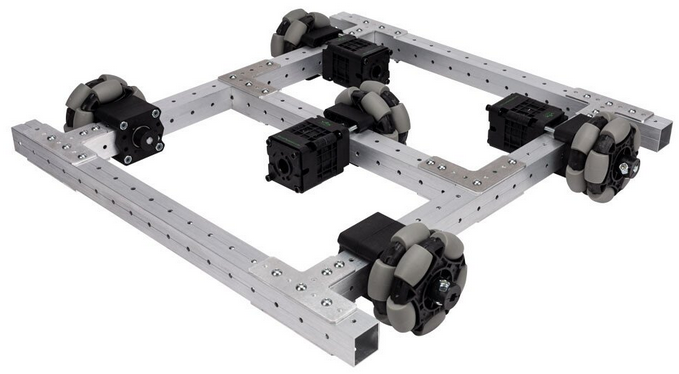
\includegraphics[height=1.7in]{imgs/drivetrain_slide.png}
	\caption{Slide}
\end{subfigure}\begin{subfigure}[b]{.45\linewidth}
	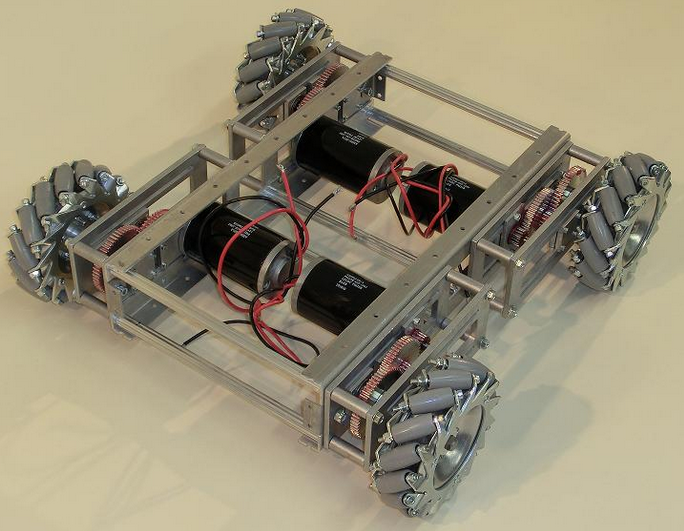
\includegraphics[height=1.7in]{imgs/drivetrain_mecanum.png}
	\caption{Mecanum}
\end{subfigure}
\caption{Omnidirectional drivetrains.}
\end{figure}

\begin{asparaenum}[a)]
	\item \textit{Kiwi drives}\index{omnidrive!kiwi} are the simplest omnidirectional drivetrain, comprised of 3 omnidirectional wheels at angles to each other. By varying the power to each wheel, movement in any axis can be produced. They are somewhat inefficient as there is a lot of slip on the rollers. \href{https://www.youtube.com/watch?v=GTRMEl4-ePc}{\color{red}\underline{Video Example}}
	\item \textit{X-drives}\index{omnidrive!x-drive} (not to be confused with 4 omni drivetrains) are like kiwi drives, but a little easier to package on rectangular frames. They benefit from a slight suspension, or at least a frame that is compliant enough to distribute weight between each wheel.
	\item \textit{H-drives}\index{omnidrive!h-drive} or \textit{slide drives}\index{omnidrive!slide-drive} are like differential drives but have a central omni wheel that enables side-to-side motion. This means that they may behave different in the side-to-side direction, but this may be an acceptable tradeoff for their higher efficiency and controllability. However, this central wheel requires a suspension system.
	\begin{figure}[H]
		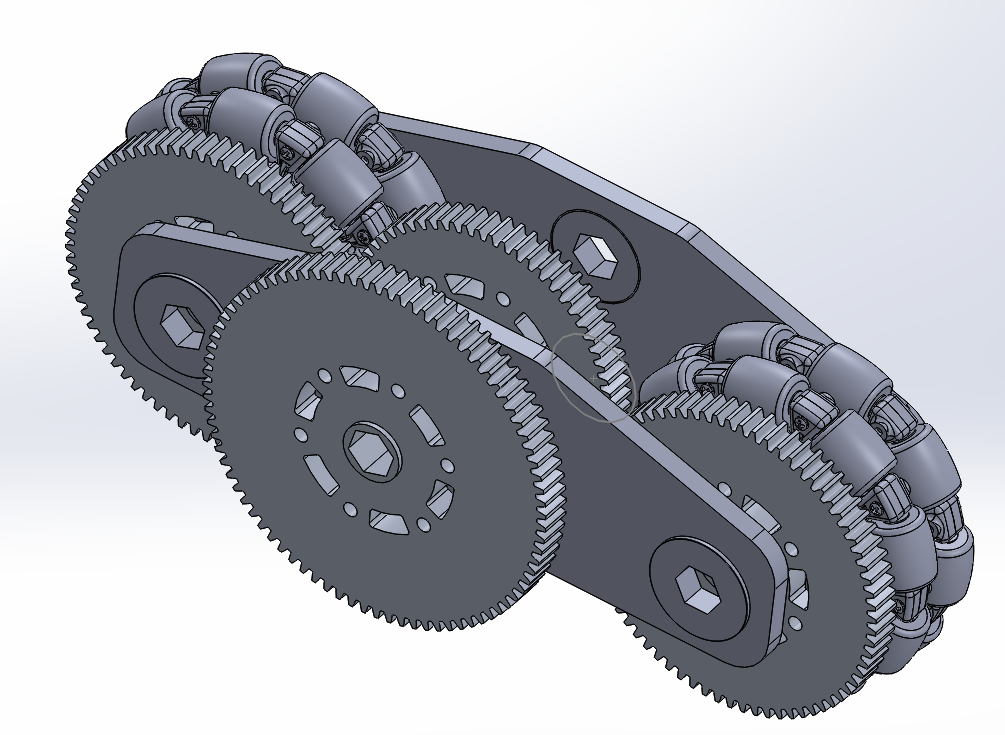
\includegraphics[width=0.7\textwidth]{imgs/drivetrain_slide_rocker.png}
		\caption{Rocker pod for a slide drive.}
	\end{figure}
	One novel suspension technique is to use not one but two wheels in a \textit{rocker pod}\index{rocker pod}. This uses the torque from the driving motor to engage the wheel with the ground, and from there, the force the wheel generates with the ground further digs the wheel into the ground. Properly setting the gear ratios can generate the proper amount of dig. \href{https://www.youtube.com/watch?v=YBUEhrsC9Es}{\color{red}\underline{Video Example}}
	\item \textit{Mecanum drives}\index{omnidrive!mecanum} use four \textit{mecanum wheels}\index{mecanum wheel}. They operate just like X-drives, but are even easier to package into rectangular frames. They are even more inefficient than x-drives, though, and have quite different behavior while strafing than moving forwards.
\end{asparaenum}

\subsection{Transformers}

\begin{figure}[H]
	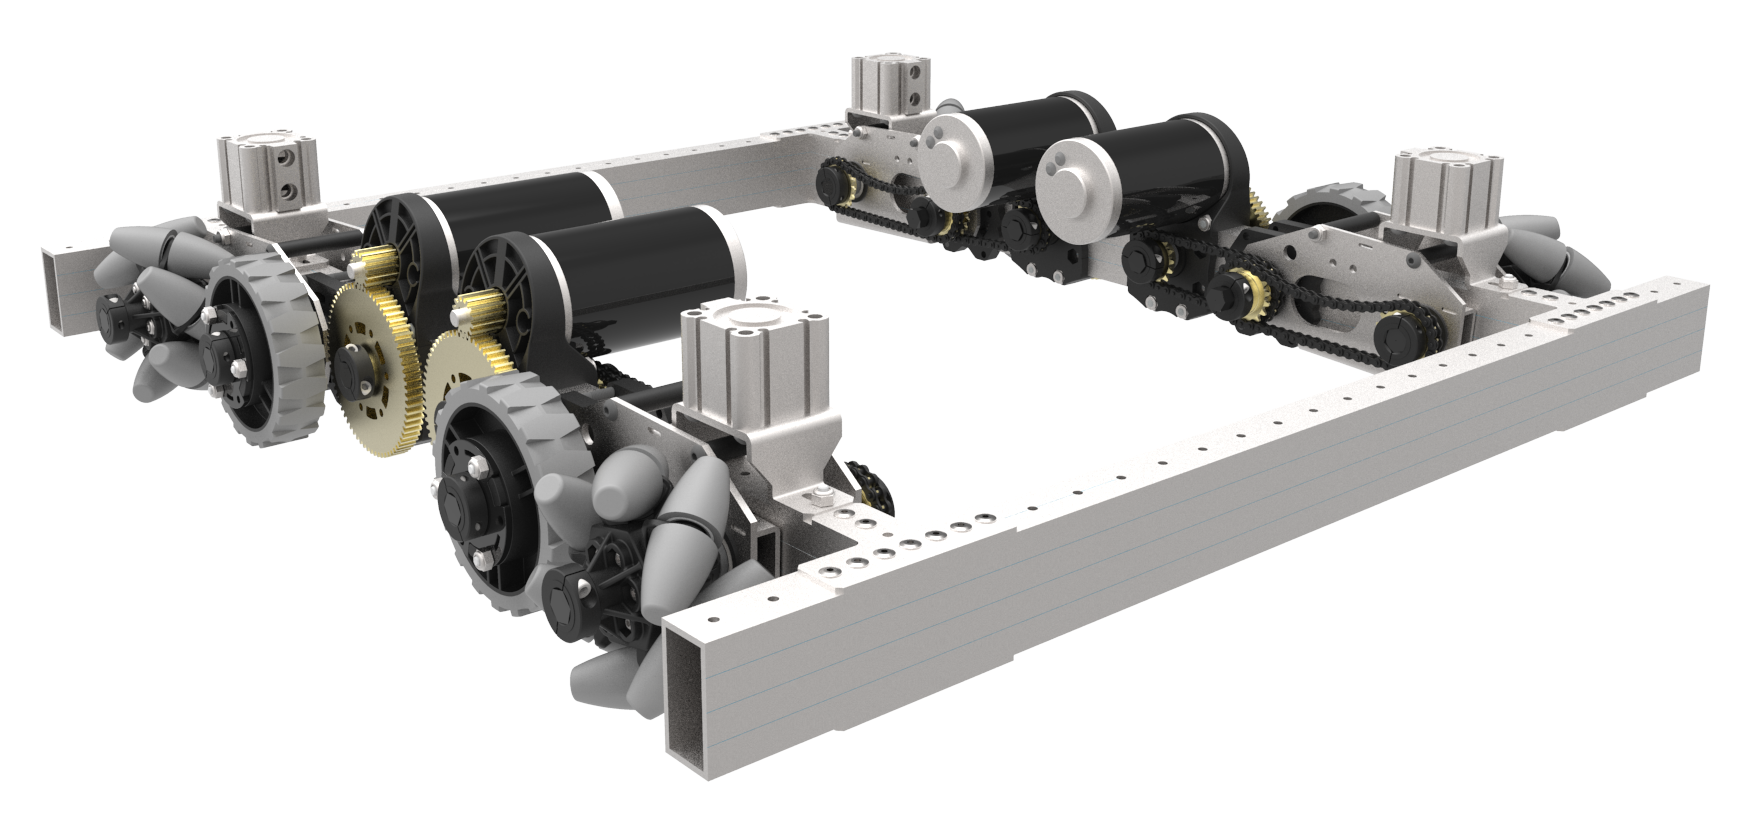
\includegraphics[width=0.8\textwidth]{imgs/drivetrain_octocanum.png}
	\caption{Octocanum drivetrain, an example of a jump drive.}
\end{figure}

\textit{Transforming}\index{Transforming} or \textit{jump}\index{jump} drives combine traditional differential drives with omni drives by taking an omni drive and chaining additional regular wheels to them which are actuated up and down. Nearly any combination can exist. but there are two general goals. First and most obvious is to enable omnidirectional motion with the choice of high-traction pushing power. The less obvious is to shift between high and low speeds since the jumped wheels can be geared at a different speed.

A jump-drive version of a mecanum drive is sometimes called an \textit{octocanum}. A jump-drive version of a slide drive is sometimes called a \textit{jump slide}. A jump-drive version of a 4 omni drivetrain (which isn't omnidirectional, just highly agile) is sometimes called a \textit{butterfly drive}.

\subsection{Fully-Steered Wheel Drives}

\textit{Swerve}\index{swerve} and \textit{crab}\index{crab drive} drives use traditional traction wheels, but steer them a full 360 degrees. This allows for simultaneous forwards-backwards, left-right, and rotational motion, but without sacrificing traction or object traversal capability like omnidrives. This comes, however, at the cost of higher mechanical and programattic complexity.

\begin{figure}[H]
\begin{subfigure}[b]{.45\linewidth}
	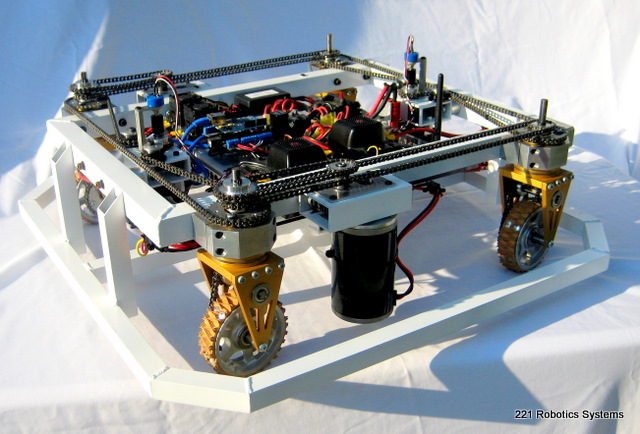
\includegraphics[height=1.7in]{imgs/drivetrain_crab.jpeg}
	\caption{Swerve}
\end{subfigure}\begin{subfigure}[b]{.45\linewidth}
	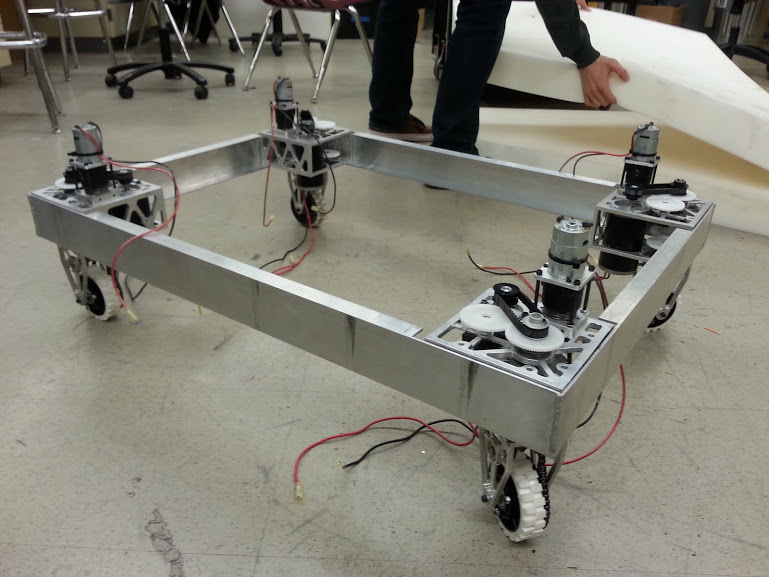
\includegraphics[height=1.7in]{imgs/drivetrain_swerve.jpeg}
	\caption{Crab}
\end{subfigure}
\caption{Swerve and crab drivetrains.}
\end{figure}

\begin{asparaenum}[a)]
	\item The wheels of \textit{crab} drives are not fully independently steered and powered. Sets of two may be steered together and then centrally powered, or some other obscure combination. This means that some wheels will not be operating at peak, and turning scrub will occur.
	\item The wheels of \textit{swerve}\index{swerve} drives are fully independently steered and powered. This means that they can all be operated at peak, but means that additional motors and sensoring is needed.
\end{asparaenum}

\begin{figure}[H]

\begin{subfigure}[b]{.32\linewidth}
	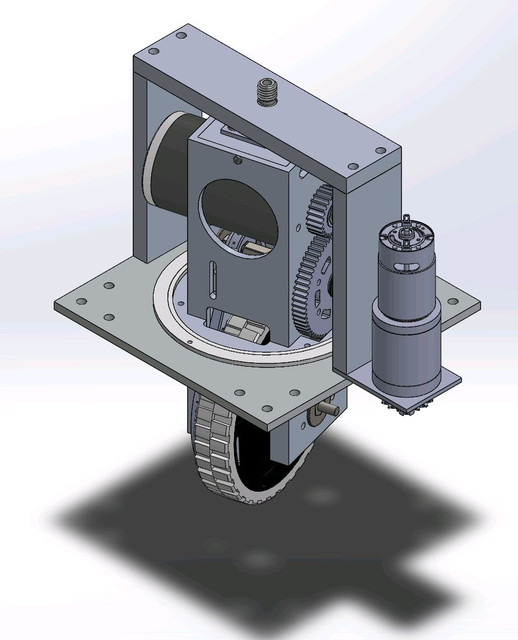
\includegraphics[height=1.7in]{imgs/drivetrain_swerve_dist.jpeg}
	\caption{Distributed (motor-in) module}
\end{subfigure}\begin{subfigure}[b]{.32\linewidth}
	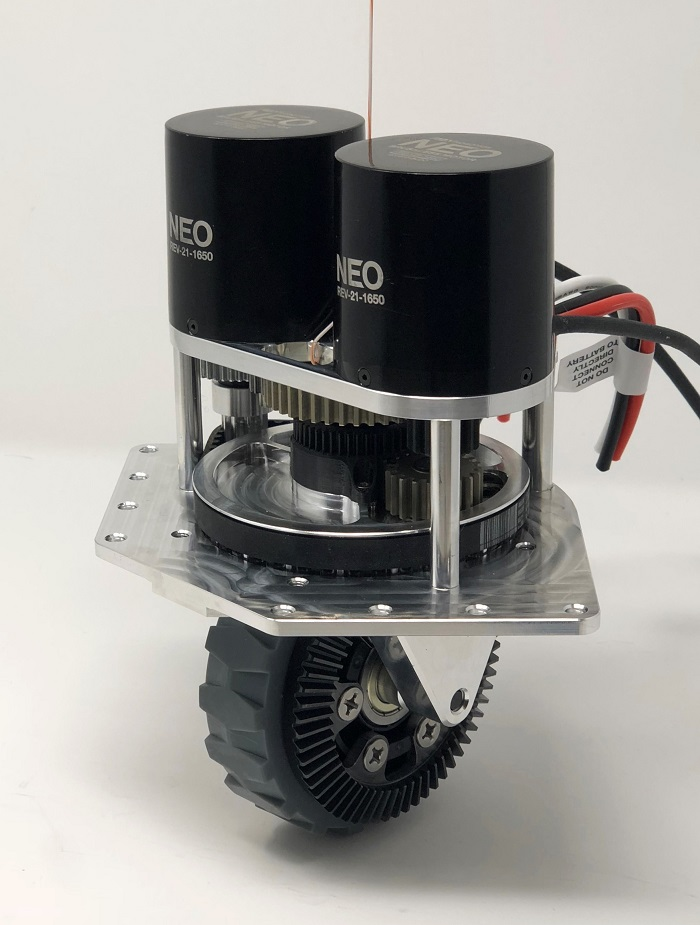
\includegraphics[height=1.7in]{imgs/drivetrain_swerve_coax.jpeg}
	\caption{Coaxial module}
\end{subfigure}\begin{subfigure}[b]{.32\linewidth}
	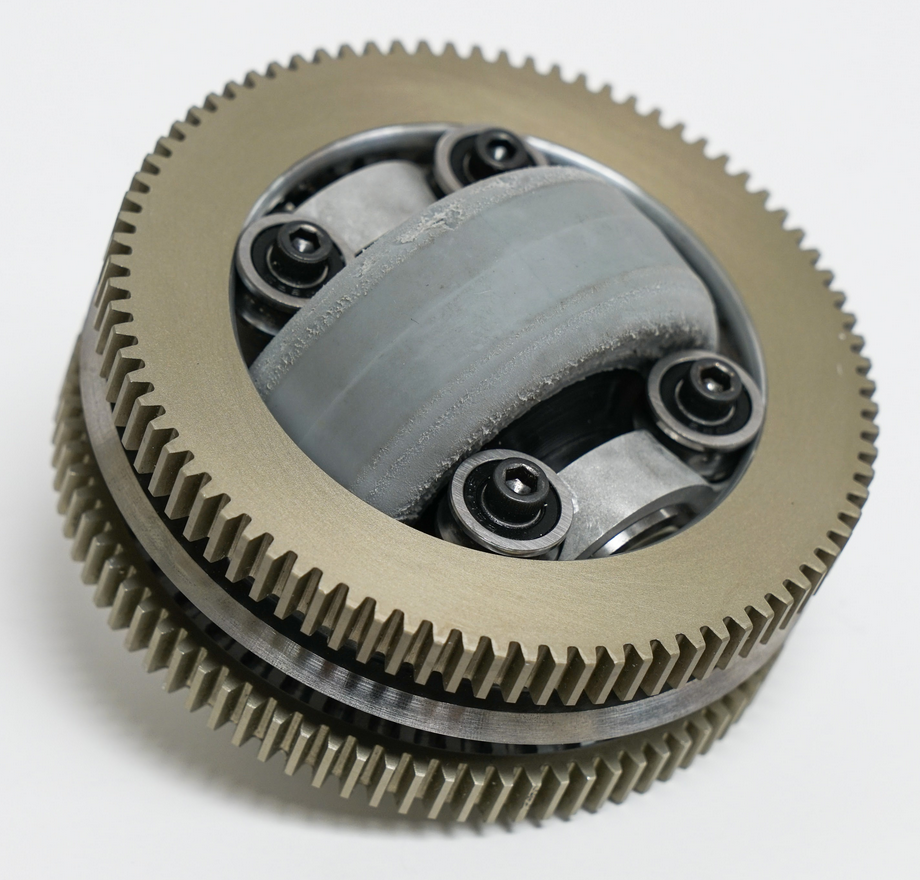
\includegraphics[height=1.7in]{imgs/drivetrain_swerve_diff.png}
	\caption{Differential}
\end{subfigure}
\caption{Swerve/crab module types.}
\end{figure}

\begin{asparaenum}[a)]
	\item \textit{Distributed}\index{swerve!distributed} modules are steered by an external motor, and have a motor in the module that spins with the module. This makes the module in some ways simpler as it does not need a bevel gear or other means to change the direction of rotation, but it does make the module quite large, and the motor's electrical wires limit the rotation of the module.
	\item \textit{Coaxial}\index{swerve!coaxial} modules are both steered and powered by an external motor.
	\item \textit{Differential}\index{swerve!differential} modules are a type of module (usually coaxial) that blends together steering and powering. Two motors are still required, but can both be utilized to create propulsive force. Additional gearing makes it such that
	\begin{align}
		T_{steering} = T_{motor, 1} - T_{motor, 2}\\
		T_{thrust}   = T_{motor, 1} + T_{motor, 2}
	\end{align}
	Many more gears are required to achieve this, but in the end, higher performance can be developed from the same number of motors/motor controllers.
\end{asparaenum}

\subsection{Addons}
Many add-on features can be added to any of these drivetrains to achieve special behavior.

\textit{Vacuum pumps}\index{vacuum} or fans can be used to forcibly remove air from the underside of a drivetrain, creating additional normal force with the ground and thusly increased grip. Notable examples are the Brabham BT46 Fan Car, and \href{https://www.youtube.com/watch?v=O9CEOHX88mw}{\color{red}\underline{FRC 95's 2020 vacuum}}- both of which were extremely powerful features, but ultimately ruled illegal. 

\begin{figure}[H]
% IMPROVEMENT: Label wheel and piston
	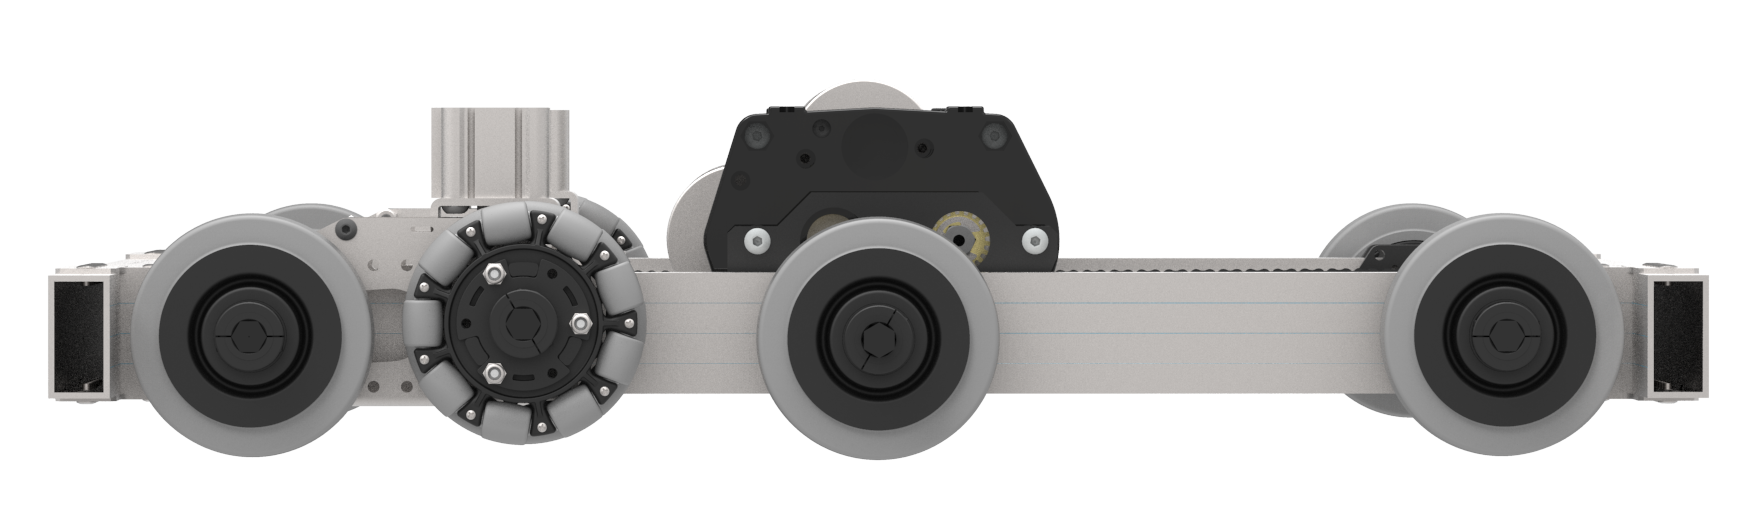
\includegraphics[width=0.95\textwidth]{imgs/drivetrain_popupwheel.png}
	\caption{Pop-down wheel on a drivetrain}
\end{figure}

\textit{Pop-down wheels}\index{pop-down wheels} are not jump drives, though they may look and behave like it at first sight. The wheel may be idle or powered, and can serve multple purposes. The first is to lift up the front wheels, enabling the drivetrain to crawl over terrain it would normally be unable to.

Pop down wheels can facilitate quick turns as illustrated in this \href{https://youtu.be/PtRewwr59d8?t=37}{\color{red}\underline{Video Example (0:37)}}.

One of the driving purposes behind pop down wheels is to help get out of \textit{friction pins}\index{friction pins}. Watch the \href{https://youtu.be/kLAkcn6l9v0?t=133}{\color{red}\underline{2011 FRC Championship Semi-Final 1 Match 1}} (match begins at 1:51, pinning begins at 2:13). 973 (in blue) is able to keep 217 (in red) from moving by pushing them in a t-bone configuration. As 217 moves sideways, their wheels lose static friction and so lose their ability to move except in an arc, which isn't an issue for 973.

Pop down wheels with omni wheels installed shift the rotation point from being in the middle of the robot (which is good for handling otherwise as the center of rotation matches the center of gravity) to being in the rear. At this point, the t-boning robot would simply push past, breaking the friction pin.

\begin{figure}[H]
	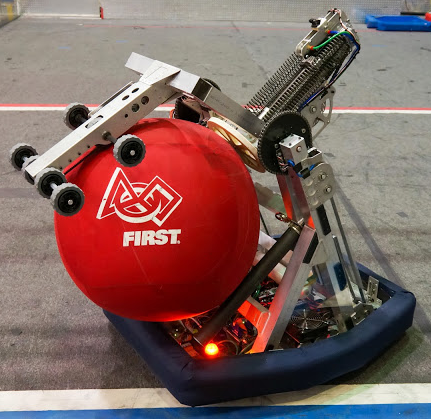
\includegraphics[width=0.6\textwidth]{imgs/drivetrain_octagon.png}
	\caption{A robot with an octagonal frame.}
\end{figure}

\textit{Curved frames}\index{curved frames} or \textit{multi-faceted frames}\index{multi-faceted frames} can also help with getting out of friction pins. These allow the pinned robot some ability to turn so they can leave the pin.

\begin{figure}[H]
	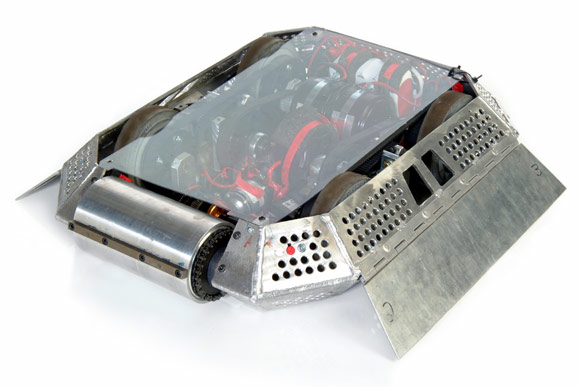
\includegraphics[width=0.6\textwidth]{imgs/drivetrain_skirt.jpeg}
	\caption{A battlebot with a skirt.}
\end{figure}

\textit{Wedge plates}\index{wedge plates} or \textit{skirts}\index{skirts} are angular plates on the exterior of a frame which can be used to get underneath other machines, stealing their normal force much like a vacuum would, and giving an advantage in pushing.